\documentclass[twocolumn]{aastex701}

\usepackage{amsmath,amssymb,mathtools}
\usepackage{graphicx}
\usepackage{booktabs}
\usepackage{array}
\usepackage{xspace}

\hypersetup{hypertexnames=false}

\shorttitle{AthenaK MHD-PIC Test Problem Description}
\shortauthors{AthenaK Collaboration}

\newcommand{\athenak}{\texttt{AthenaK}\xspace}
\newcommand{\pic}{\texttt{PIC}\xspace}
\newcommand{\mhd}{\texttt{MHD}\xspace}
\newcommand{\task}[1]{\textbf{Task #1}}
\newcommand{\logic}[1]{\textit{Logic.} #1}
\newcommand{\result}[1]{\textit{Result.} #1}
\newcommand{\implication}[1]{\textit{Implication.} #1}
\newcommand{\nextstep}[1]{\textit{Next step.} #1}

\begin{document}

\title{AthenaK MHD-PIC Test Problem Description and Validation Atlas (Internal Draft)}

\author{AthenaK Collaboration}
\affiliation{Internal Methods Note}
\email{athenak-dev@local}

\begin{abstract}
This document is a method-facing atlas of the current \athenak test-problem
suite for \mhd, stand-alone \pic, and coupled MHD-PIC workflows. We organize
the material as one task per test, then describe each task in a common four-part
structure: what it tests, what the present result is, what that result implies,
and what upgrade is still worth doing.

The figure set mixes quantitative diagnostics (convergence curves, growth-mode
histories, anisotropy slopes, and drift traces) with state visualizations
(particle-support maps and shock-structure panels). The core message is
practical: the suite already establishes broad implementation credibility, but
the highest-impact CR-shock storyline and several instability windows still
require targeted redesign before final publication claims.
\end{abstract}

\section{Scope and Reading Strategy}

The purpose of this paper is straightforward: make the test suite legible enough
that a reader can move from code-level checks to physics-level confidence
without guessing what each gate is actually proving. We therefore keep the
mapping explicit. Every task description includes:
\begin{enumerate}
\item the \textit{logic} of the test,
\item the present \textit{result},
\item the practical \textit{implication}, and
\item an optional \textit{next step} when the current result is not yet
science-grade.
\end{enumerate}

The catalog and naming are aligned with
\texttt{AGENT\_PIC\_TEST\_PROBLEM\_CATALOG.md}. This note is an internal
methods draft; it is not a final science-results paper.

\section{Task List: One Test Problem Per Task}

\subsection{Complete Task Index (Current)}

\begin{enumerate}
\item \task{1}: \texttt{hydro.hydro\_linwave}
\item \task{2}: \texttt{mhd.mhd\_linwave}
\item \task{3}: \texttt{mhd.divb\_amr}
\item \task{4}: \texttt{particles.pic\_entity\_deposit\_mink}
\item \task{5}: \texttt{particles.pic\_entity\_deposit\_reflect}
\item \task{6}: \texttt{particles.pic\_em\_vacuum\_wave}
\item \task{7}: \texttt{particles.pic\_langmuir\_frequency\_proxy}
\item \task{8}: \texttt{particles.pic\_two\_stream\_growth\_proxy}
\item \task{9}: \texttt{particles.pic\_weibel\_growth\_proxy}
\item \task{10}: \texttt{particles.pic\_no\_mhd\_boris}
\item \task{11}: \texttt{particles.pic\_boris\_midpoint\_eb}
\item \task{12}: \texttt{particles.pic\_bell\_growth\_proxy}
\item \task{13}: \texttt{particles.pic\_multispecies\_backreaction\_oscillation}
\item \task{14}: \texttt{particles.pic\_crsi\_deltaf\_proxy}
\item \task{15}: \texttt{particles.pic\_crpai\_polarization\_proxy}
\item \task{16}: \texttt{particles.pic\_expanding\_box\_anisotropy\_proxy}
\item \task{17}: \texttt{particles.pic\_refinement\_boundary\_characterization}
\item \task{18}: \texttt{particles.pic\_amr\_shock\_lb\_smoke}
\item \task{19}: \texttt{particles.pic\_analysis\_utils}
\item \task{20}: \texttt{particles.pic\_deposit\_conservation}
\item \task{21}: \texttt{particles.pic\_decomp\_invariance}
\item \task{22}: \texttt{particles.pic\_mhd\_passive\_mode}
\item \task{23}: \texttt{particles.pic\_mhd\_current\_coupling}
\item \task{24}: \texttt{particles.pic\_mhd\_coupling\_decomp}
\item \task{25}: \texttt{particles.pic\_mhd\_coupling\_multilevel}
\item \task{26}: \texttt{particles.pic\_mhd\_coupling\_nonperiodic}
\item \task{27}: \texttt{particles.pic\_mhd\_restart\_fidelity}
\item \task{28}: \texttt{particles.pic\_restart\_safety\_guards}
\end{enumerate}

\section{Baseline Hydro and MHD Tasks (Tasks 1--3)}

These three tasks are deliberately conservative. If they drift, every later
particle claim becomes ambiguous.

\subsubsection*{Task 1: \texttt{hydro\_linwave}}
\textbf{Setup:} script \texttt{hydro\_linwave.py}; input deck
\texttt{linear\_wave\_hydro.athinput}. \logic{The test isolates pure
hydrodynamic wave transport and asks whether L1 errors fall cleanly with
resolution across hydro solver options.} \result{The gate remains a stable
convergence check in the suite and provides order-of-accuracy trends for the
hydro branches.} \implication{Hydrodynamic transport remains a trustworthy base
layer for later PIC coupling work.} \nextstep{Add a compact publication panel
for this task so the baseline is visible in the same figure bundle as the PIC
results.}

\subsubsection*{Task 2: \texttt{mhd\_linwave}}
\textbf{Setup:} script \texttt{mhd\_linwave.py}; input deck
\texttt{linear\_wave\_mhd.athinput}. \logic{The test probes fast,
Alfv\'en, slow, and entropy branches to verify that MHD wave families converge
without branch-specific pathology.} \result{Current gating continues to report
clean L1 behavior across the branch set.} \implication{The core MHD transport
operator remains credible, so instability and coupling behavior in later tests
is less likely to be contaminated by baseline wave errors.} \nextstep{Expose a
small multi-branch summary plot in the publication bundle to make this evidence
directly visible.}

\subsubsection*{Task 3: \texttt{divb\_amr}}
\textbf{Setup:} script \texttt{divb\_amr.py}; input deck
\texttt{ffc\_divb.athinput}. \logic{This task stress-tests constrained
transport under AMR by enforcing a strict divergence-cleanliness threshold.}
\result{The gate enforces $\max(|\nabla\cdot\mathbf{B}|) < 10^{-10}$ on AMR
outputs and remains the strongest scalar health check for magnetic consistency
with refinement.} \implication{When later coupled tests show structure changes,
those changes are less likely to be numerical monopoles in disguise.}
\nextstep{Add a time-history diagnostic of $\nabla\cdot\mathbf{B}$ extrema to
show whether cleanliness is merely bounded or actively damped.}

\section{Entity-Mirroring PIC Core Tasks (Tasks 4--9)}

This block asks a simple question: does AthenaK reproduce the core deposition,
wave, and instability signatures expected from the Entity-style reference logic?

\begin{figure*}[htbp]
\centering
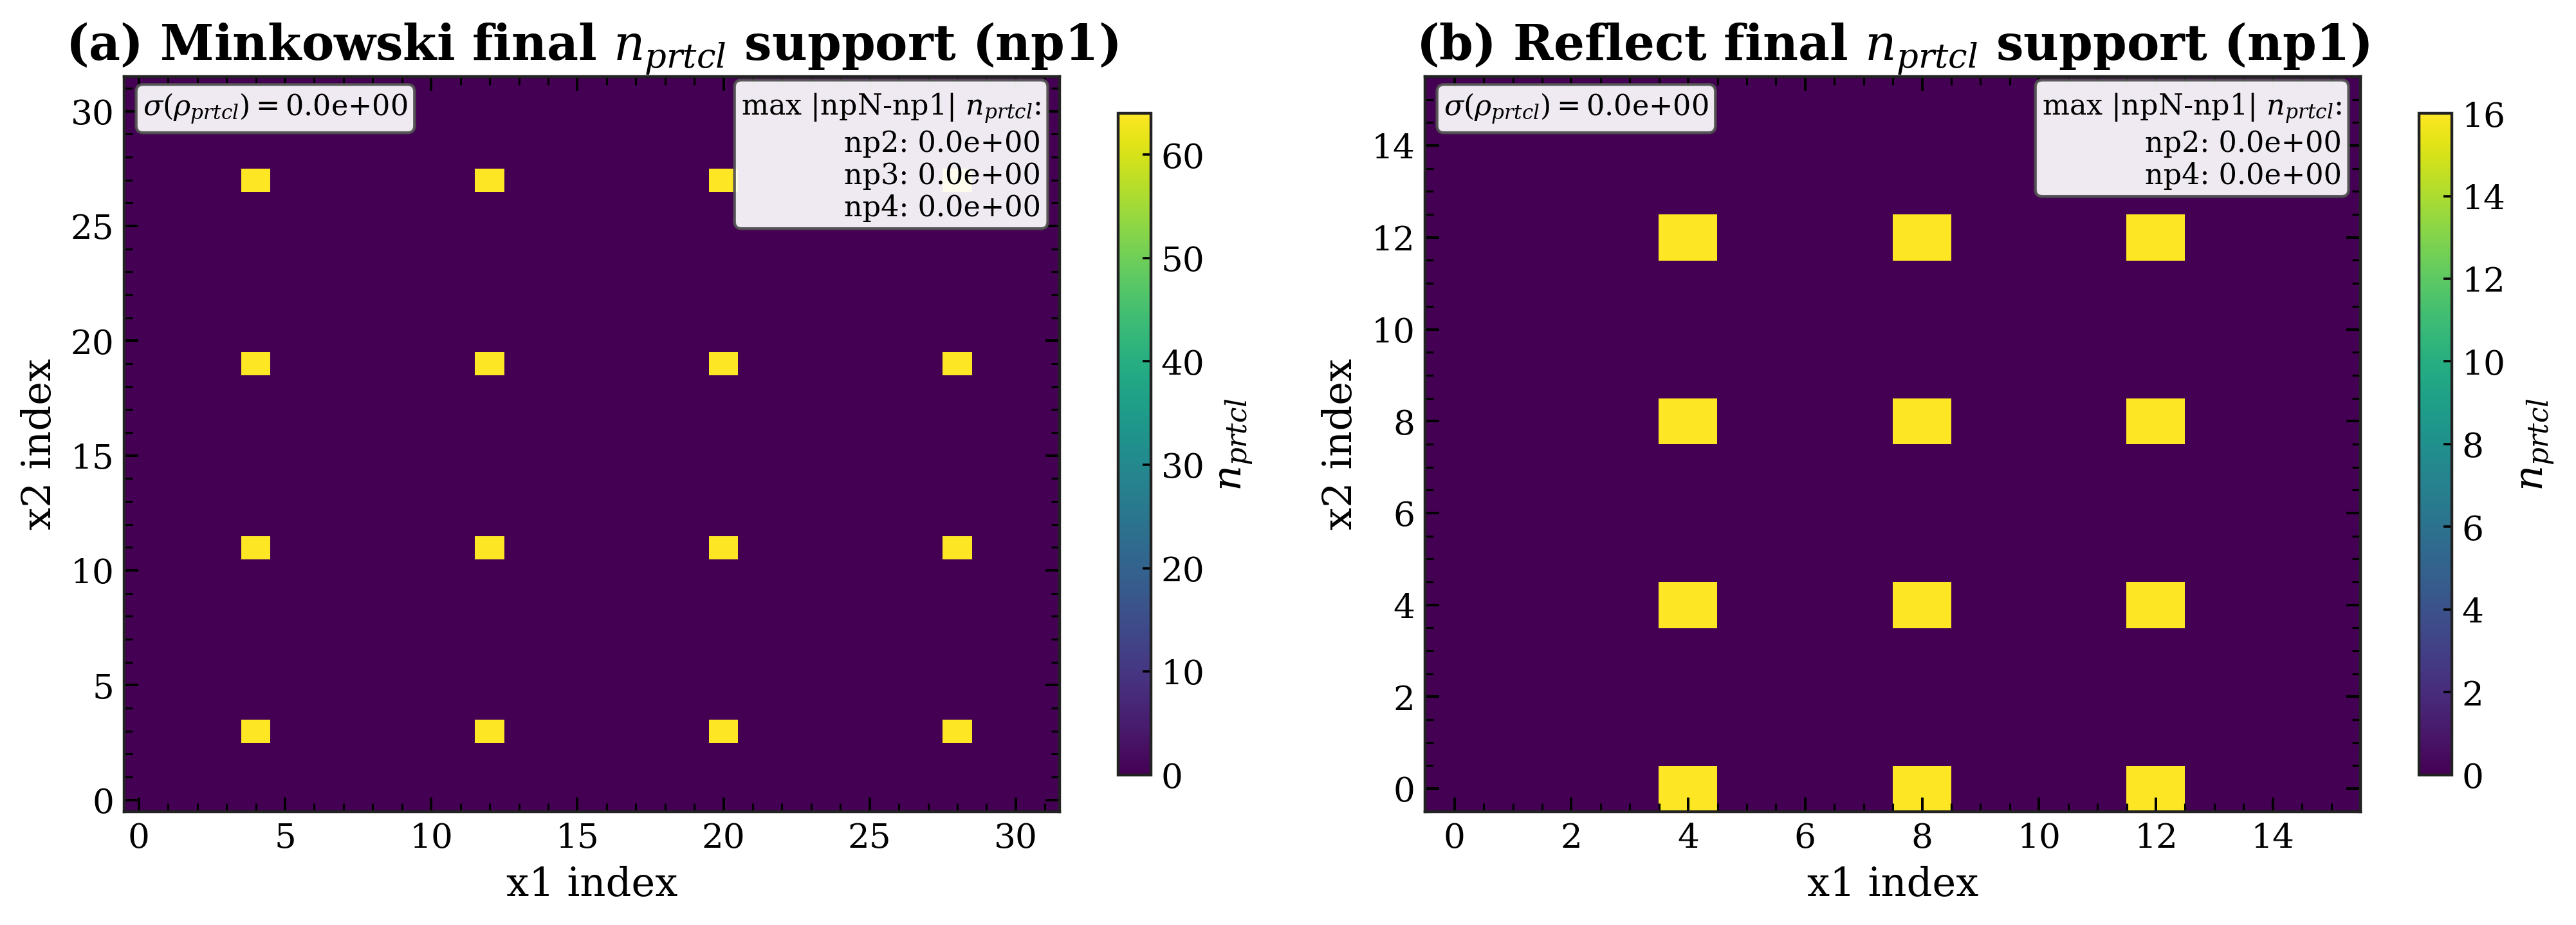
\includegraphics[width=0.98\textwidth]{figures/01_entity_deposit_maps.png}
\caption{Entity-mirroring deposit support maps for Minkowski and reflecting
configurations (Task 4 and Task 5). Bright cells mark the particle-support
stencil. Annotations report support variance and decomposition differences; in
this generated set those differences are zero at the plotted precision.}
\label{fig:entity-deposit}
\end{figure*}

\subsubsection*{Task 4: \texttt{pic\_entity\_deposit\_mink}}
\textbf{Setup:} script \texttt{pic\_entity\_deposit\_mink.py}; input deck
\texttt{pic\_entity\_deposit\_mink.athinput}. \logic{The test checks charge,
current, and particle-support parity for a Minkowski-style deposition stencil.}
\result{Figure~\ref{fig:entity-deposit} (left) shows an identical support map
across ranks, with zero reported support variance and zero
$|\mathrm{npN}-\mathrm{np1}|$ differences at the displayed precision.}
\implication{The discrete deposition geometry is decomposition-invariant in this
configuration, which is a precondition for credible MPI scaling studies.}
\nextstep{Expand this task with an off-grid phase sweep so parity is tested away
from highly symmetric particle placements.}

\subsubsection*{Task 5: \texttt{pic\_entity\_deposit\_reflect}}
\textbf{Setup:} script \texttt{pic\_entity\_deposit\_reflect.py}; input deck
\texttt{pic\_entity\_deposit\_reflect.athinput}. \logic{This variant probes
whether reflecting boundaries preserve the same deposition integrity as periodic
or free-space cases.} \result{Figure~\ref{fig:entity-deposit} (right) shows the
expected reflected support pattern with the same decomposition agreement seen in
Task 4.} \implication{Boundary treatment is not introducing rank-dependent
artifacts in the measured support stencil.} \nextstep{Add a moving-particle
reflection sequence to check parity through boundary crossings, not only at a
single snapshot.}

\begin{figure}[htbp]
\centering
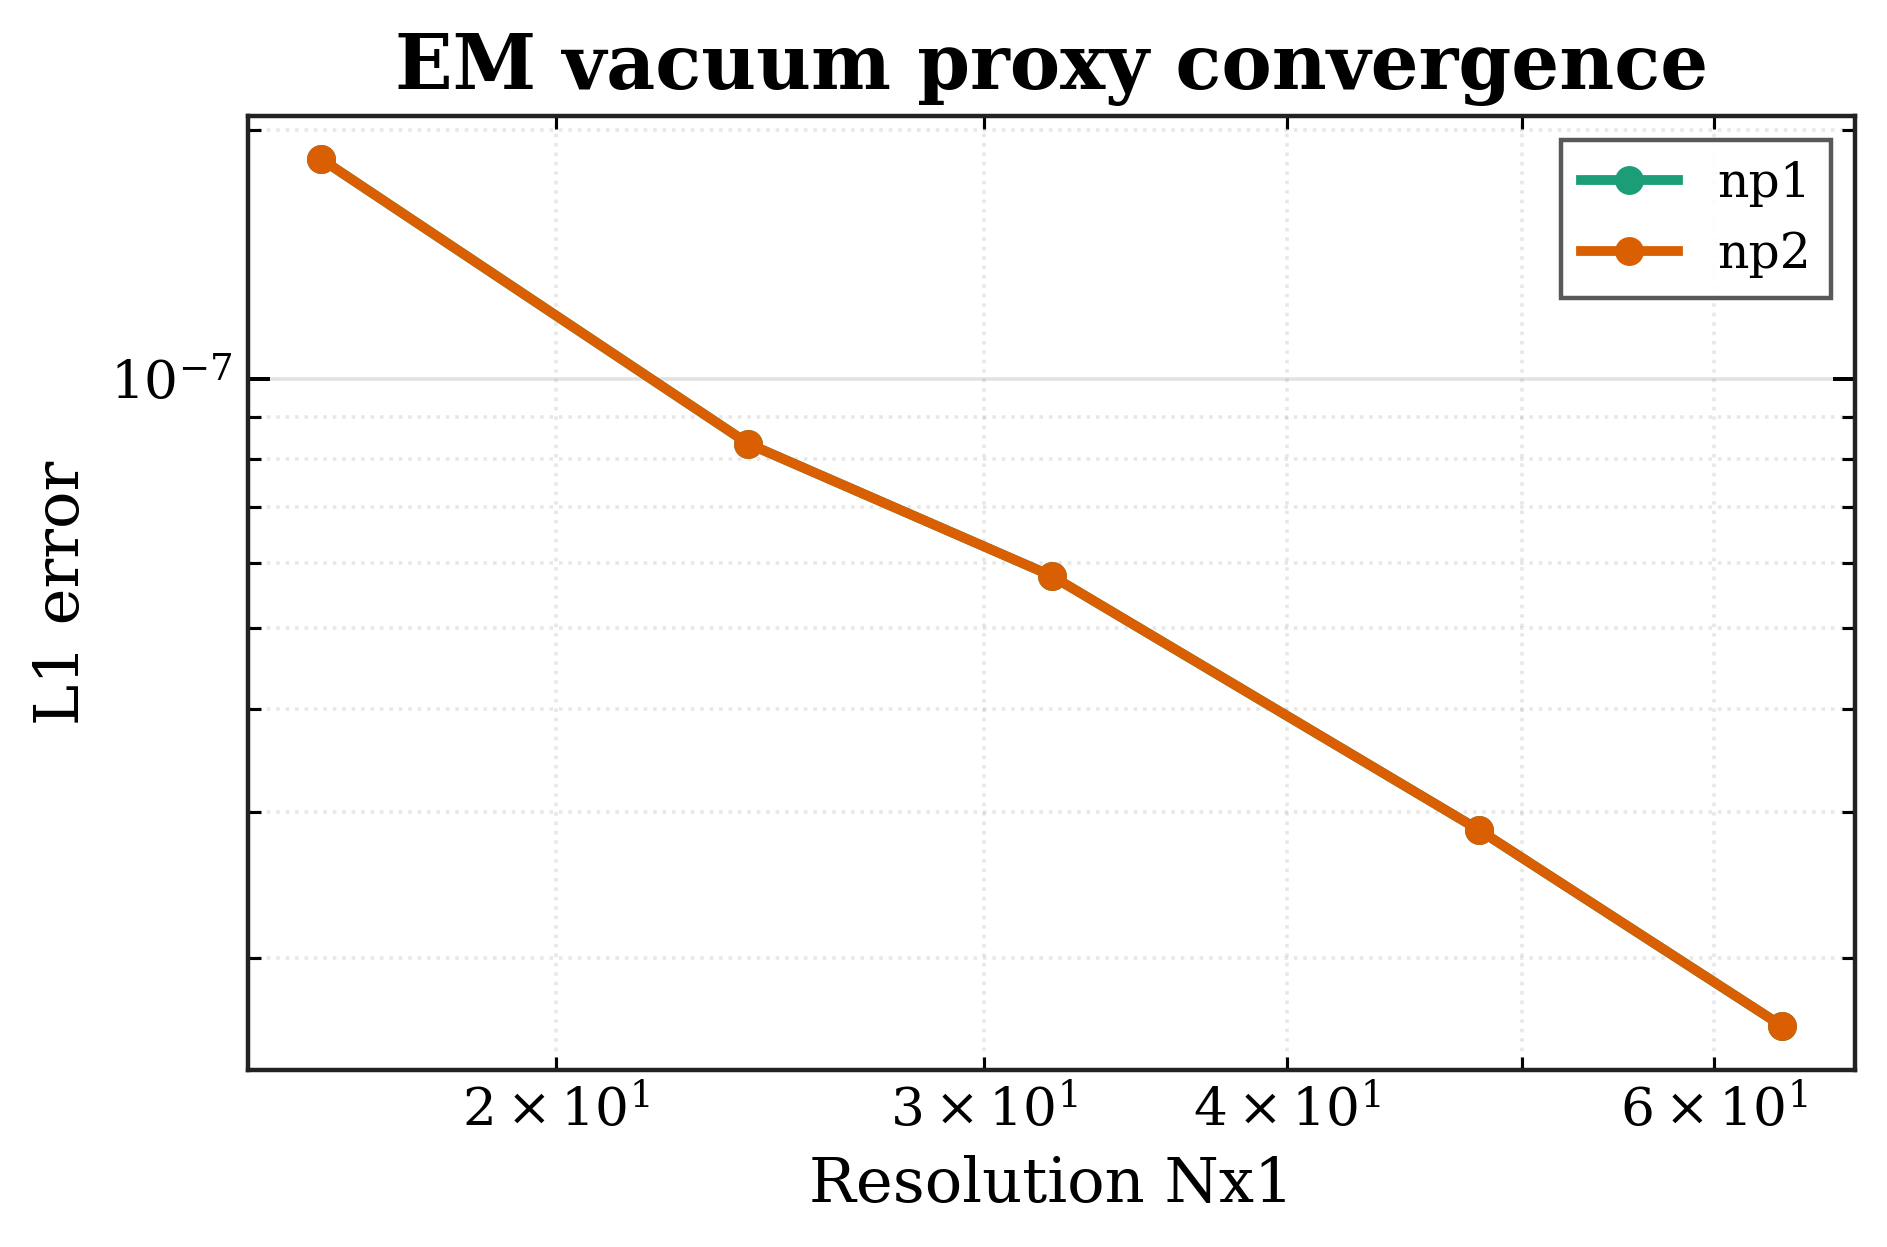
\includegraphics[width=\columnwidth]{figures/02_em_vacuum_convergence.png}
\caption{EM-vacuum convergence (Task 6) with serial and MPI overlays. The two
curves are visually coincident while L1 error decreases with increasing
resolution, indicating decomposition invariance and expected convergence
behavior.}
\label{fig:em-vacuum}
\end{figure}

\subsubsection*{Task 6: \texttt{pic\_em\_vacuum\_wave}}
\textbf{Setup:} script \texttt{pic\_em\_vacuum\_wave.py}; input deck
\texttt{pic\_em\_vacuum\_wave.athinput}. \logic{The task checks whether
vacuum EM propagation remains accurate when evolved through the PIC field
machinery.} \result{Figure~\ref{fig:em-vacuum} shows monotonic error reduction
across the tested resolutions and a near-perfect serial/MPI overlay.}
\implication{The field update and decomposition pipeline preserve both
consistency and convergence in the linear vacuum limit.} \nextstep{Increase the
resolution ladder by one or two points to make formal order fits more stable.}

\begin{figure*}[htbp]
\centering
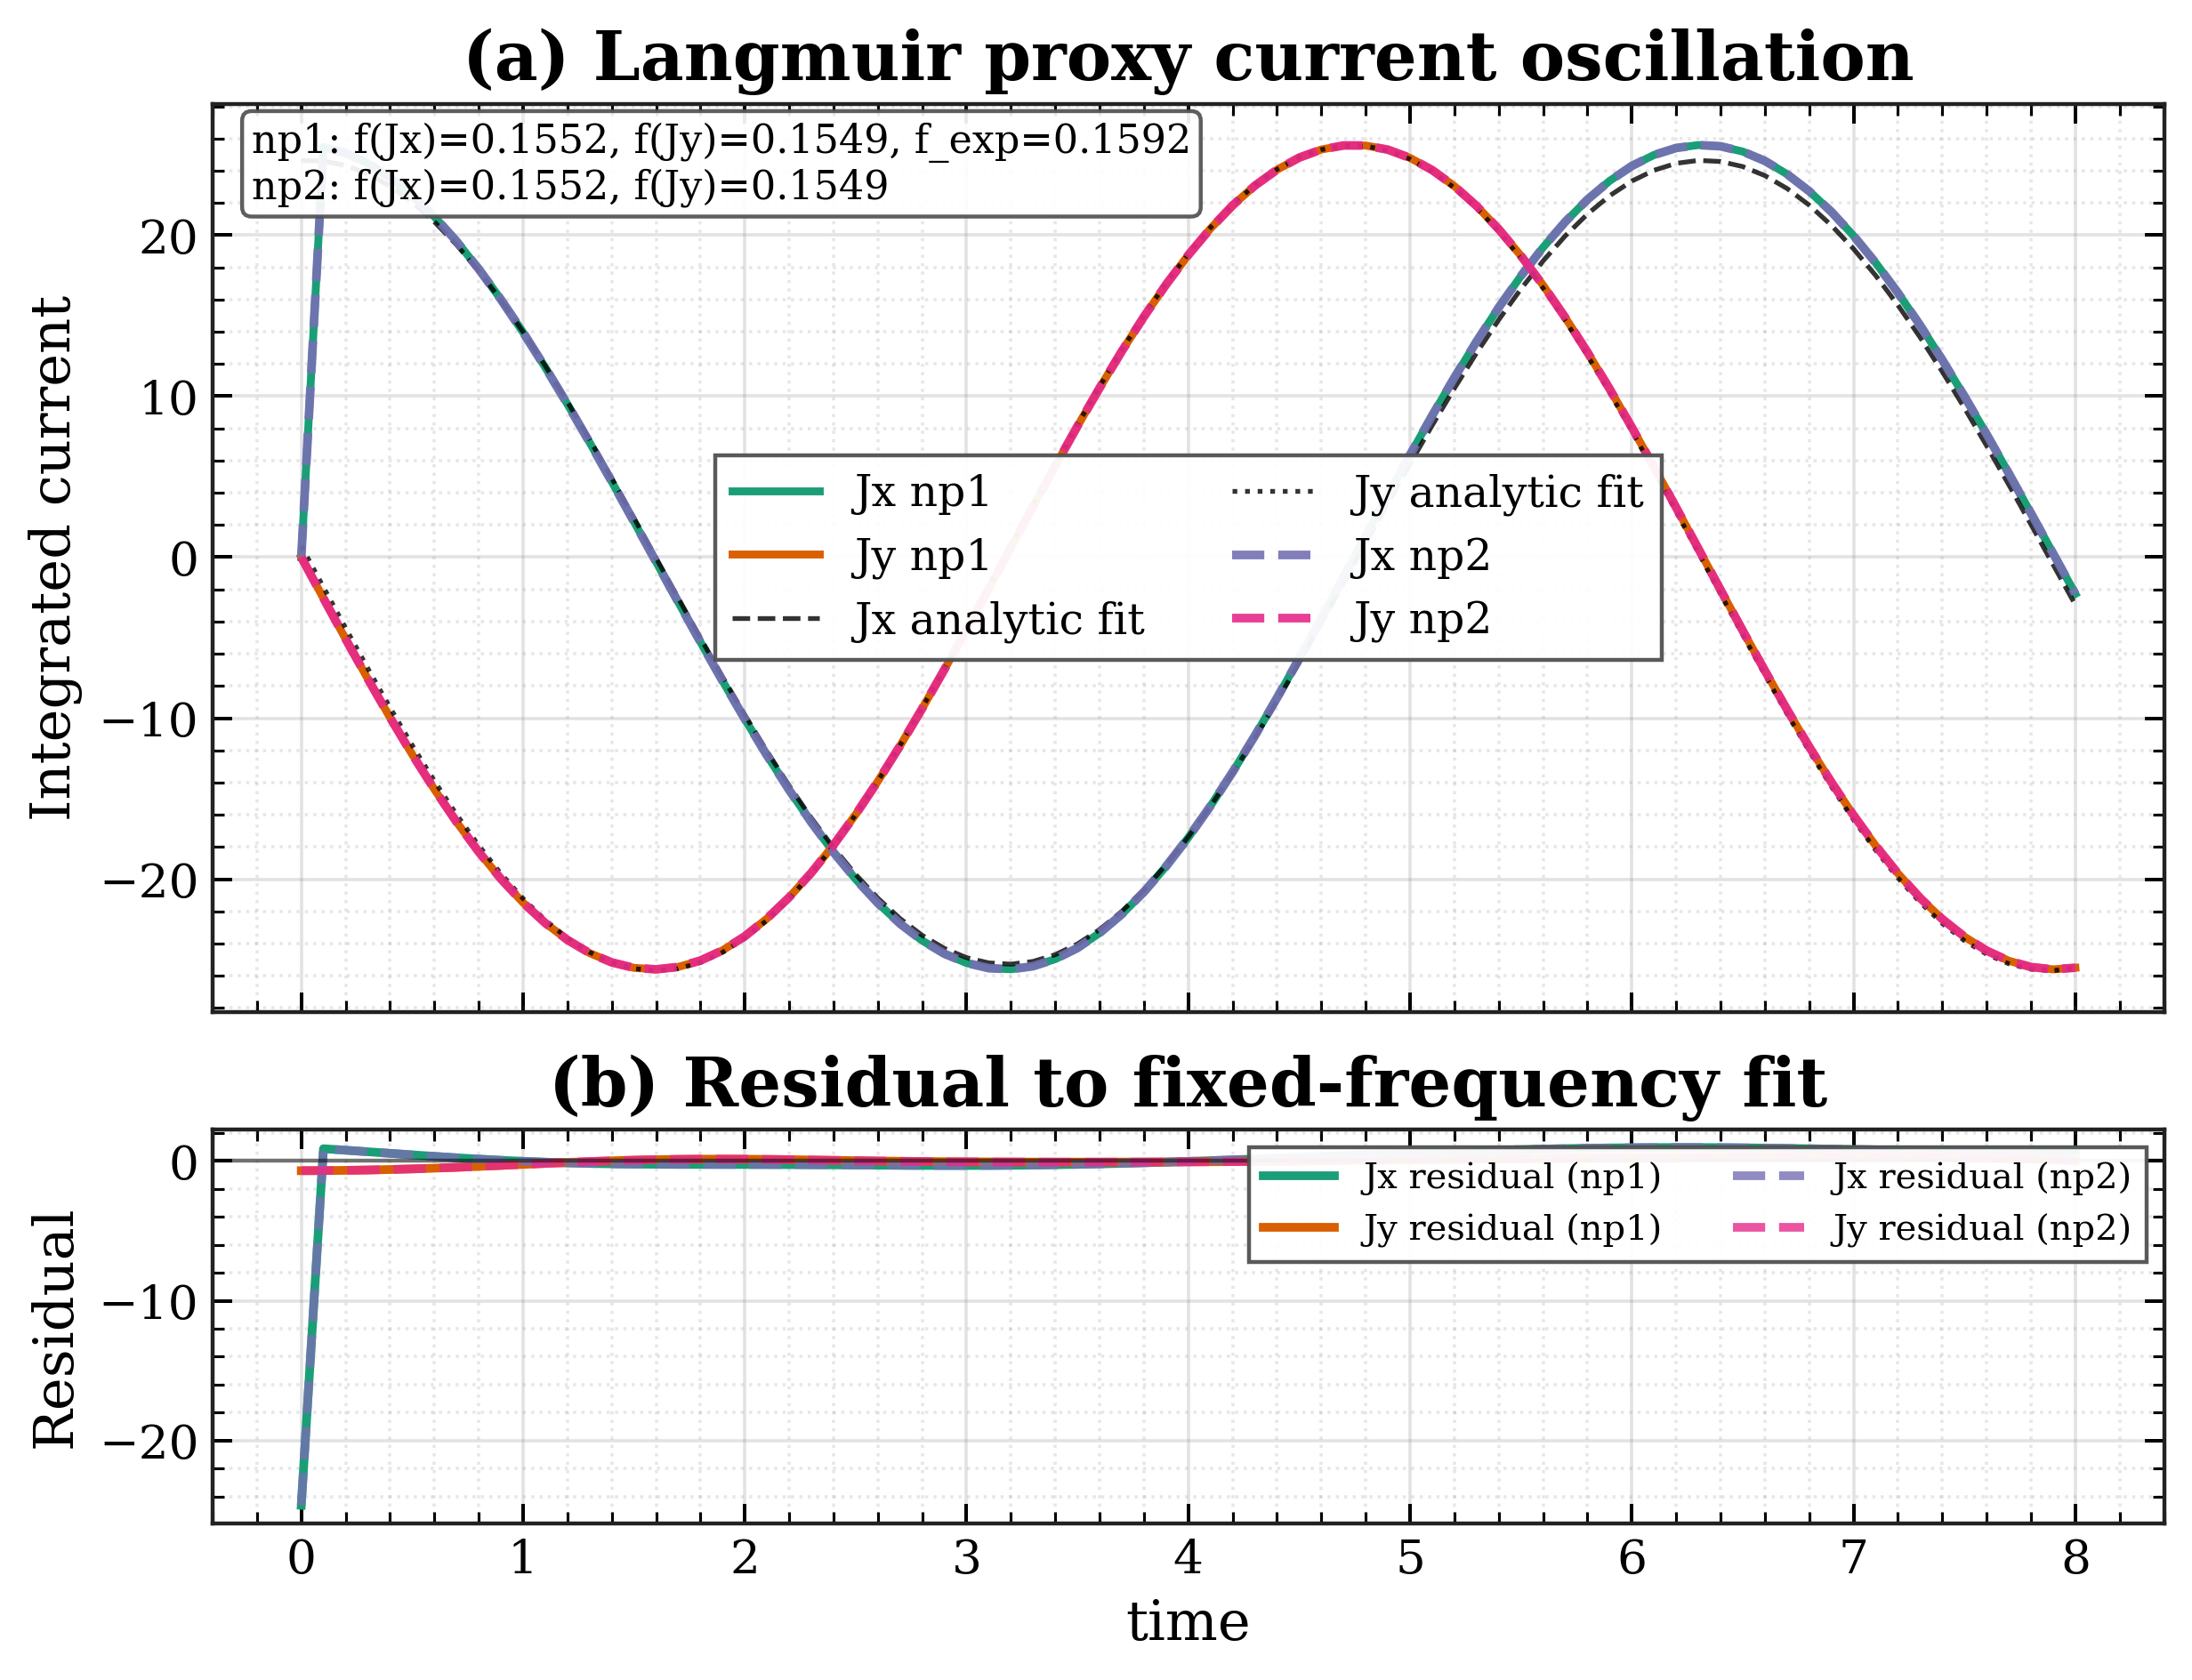
\includegraphics[width=0.95\textwidth]{figures/03_langmuir_currents.png}
\caption{Langmuir-current oscillation and residuals (Task 7). Top panel:
integrated $J_x$ and $J_y$ with fixed-frequency analytic fits. Bottom panel:
residual to that fit. The dominant recovered frequencies are close to the proxy
target and remain aligned between serial and MPI runs.}
\label{fig:langmuir}
\end{figure*}

\subsubsection*{Task 7: \texttt{pic\_langmuir\_frequency\_proxy}}
\textbf{Setup:} script \texttt{pic\_langmuir\_frequency\_proxy.py}; input deck
\texttt{pic\_langmuir\_frequency\_proxy.athinput}. \logic{Rather than merely
checking sinusoidal shape, this task checks whether the current history recovers
the intended plasma frequency.} \result{The fitted frequencies in the current
panel are close to the expected proxy value and serial/MPI traces are
indistinguishable over most of the window.} \implication{The pusher+deposition
path reproduces the intended oscillation timescale in this controlled regime.}
\nextstep{Reduce the startup transient (large first-step residual) with a
ramped initialization so frequency fits rely on cleaner early-time data.}

\begin{figure*}[htbp]
\centering
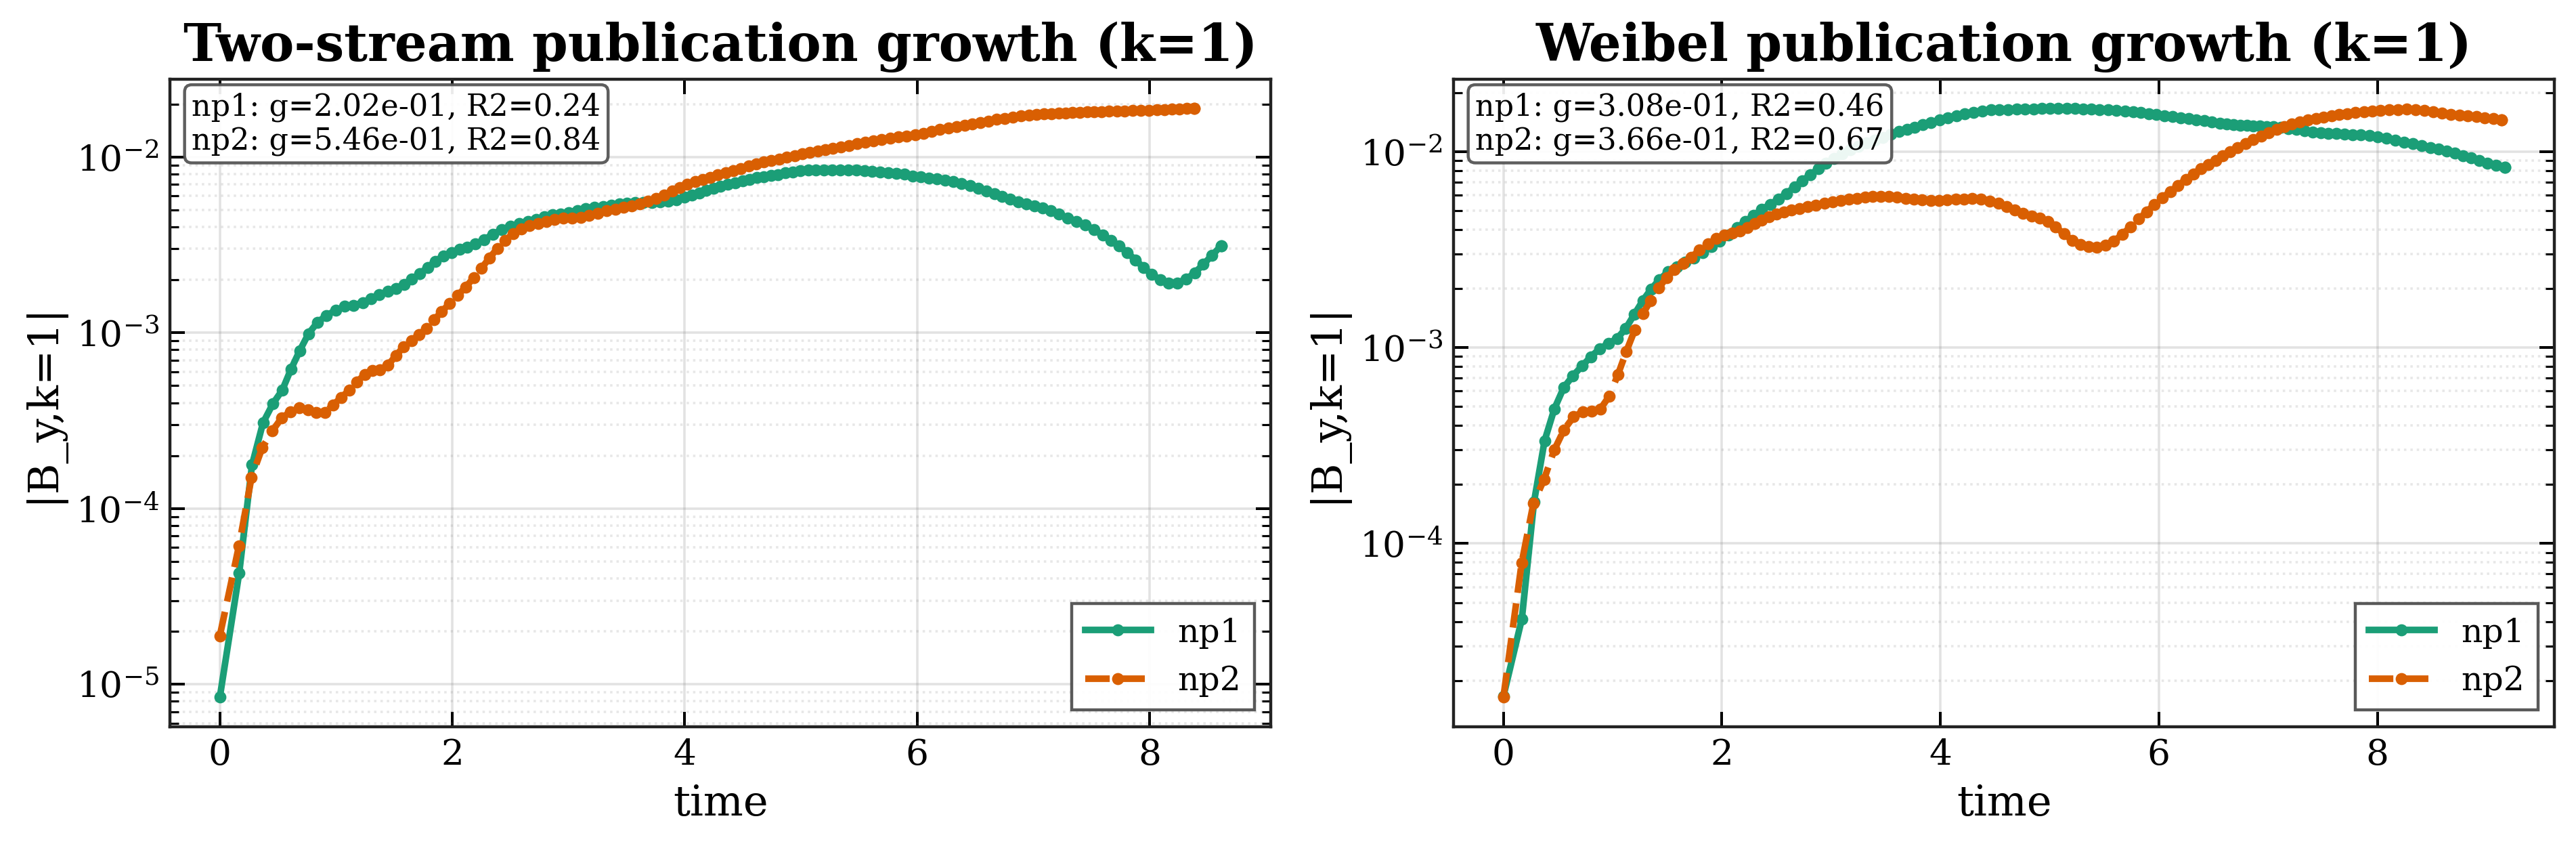
\includegraphics[width=0.98\textwidth]{figures/04_two_stream_weibel_modes.png}
\caption{Two-stream and Weibel publication-growth proxies (Tasks 8 and 9).
Mode amplitudes are shown on log scales with rank overlays. Both tasks display
early growth and later nonlinear shaping, with rank consistency in trend but not
perfect overlap in every phase of the trajectory.}
\label{fig:twostream-weibel}
\end{figure*}

\subsubsection*{Task 8: \texttt{pic\_two\_stream\_growth\_proxy}}
\textbf{Setup:} script \texttt{pic\_two\_stream\_growth\_proxy.py}; input deck
\texttt{pic\_two\_stream\_growth\_proxy.athinput}. \logic{The task targets
unstable electrostatic mode amplification with decomposition-robust behavior.}
\result{Figure~\ref{fig:twostream-weibel} (left) shows strong early growth from
low amplitude into a nonlinear envelope, with rank-consistent onset but modest
late-window divergence.} \implication{The instability trigger is present and
robust, but the sampled window mixes linear and nonlinear phases, so simple
single-slope fits are not fully diagnostic.} \nextstep{Retune this proxy to
hold a longer clean linear window before saturation for publication-grade growth
rate extraction.}

\subsubsection*{Task 9: \texttt{pic\_weibel\_growth\_proxy}}
\textbf{Setup:} script \texttt{pic\_weibel\_growth\_proxy.py}; input deck
\texttt{pic\_weibel\_growth\_proxy.athinput}. \logic{The task probes magnetic
mode amplification in a Weibel-like proxy configuration.} \result{Figure
\ref{fig:twostream-weibel} (right) shows clear growth and rank-tracked trend
agreement, again with nonlinear shaping over the longer interval.}
\implication{The solver captures the expected instability pathway, but the
present setup is a credibility proxy rather than a final dispersion-relation
measurement.} \nextstep{Add short-window linear-fit reporting with confidence
intervals to separate onset physics from saturation morphology.}

\section{Athena++-Inspired MHD-PIC Benchmark Tasks (Tasks 10--18)}

This section moves from core PIC mechanics into CR-coupled behavior inspired by
the Athena++ MHD-PIC benchmark logic. The central question is no longer ``does
it run,'' but ``does it run in the right physical direction, with transparent
limits?''

\subsubsection*{Task 10: \texttt{pic\_no\_mhd\_boris}}
\textbf{Setup:} script \texttt{pic\_no\_mhd\_boris.py}; input deck
\texttt{pic\_no\_mhd\_boris.athinput}. \logic{This is the clean single-particle
orbit baseline that isolates pusher behavior from MHD coupling effects.}
\result{The gate remains a stable invariant/safety check and is used as a
reference for later coupled pusher diagnostics.} \implication{When coupled runs
show drift or phase error, Task 10 helps separate pusher defects from coupling
side effects.} \nextstep{Expose one compact orbit-and-invariant figure in the
main bundle so this baseline is visually auditable.}

\subsubsection*{Task 11: \texttt{pic\_boris\_midpoint\_eb}}
\textbf{Setup:} script \texttt{pic\_boris\_midpoint\_eb.py}; input deck
\texttt{pic\_boris\_midpoint\_eb.athinput}. \logic{The task verifies the
midpoint E+B staging used in the modernized pusher path and checks frozen-in
consistency under staged updates.} \result{Current gating confirms expected
momentum/energy-exchange behavior for this controlled setup.}
\implication{The midpoint formulation is integrated coherently with the
operator-splitting sequence used by coupled updates.} \nextstep{Add an explicit
error-versus-step-size curve to quantify pusher convergence rate in this mode.}

\begin{figure}[htbp]
\centering
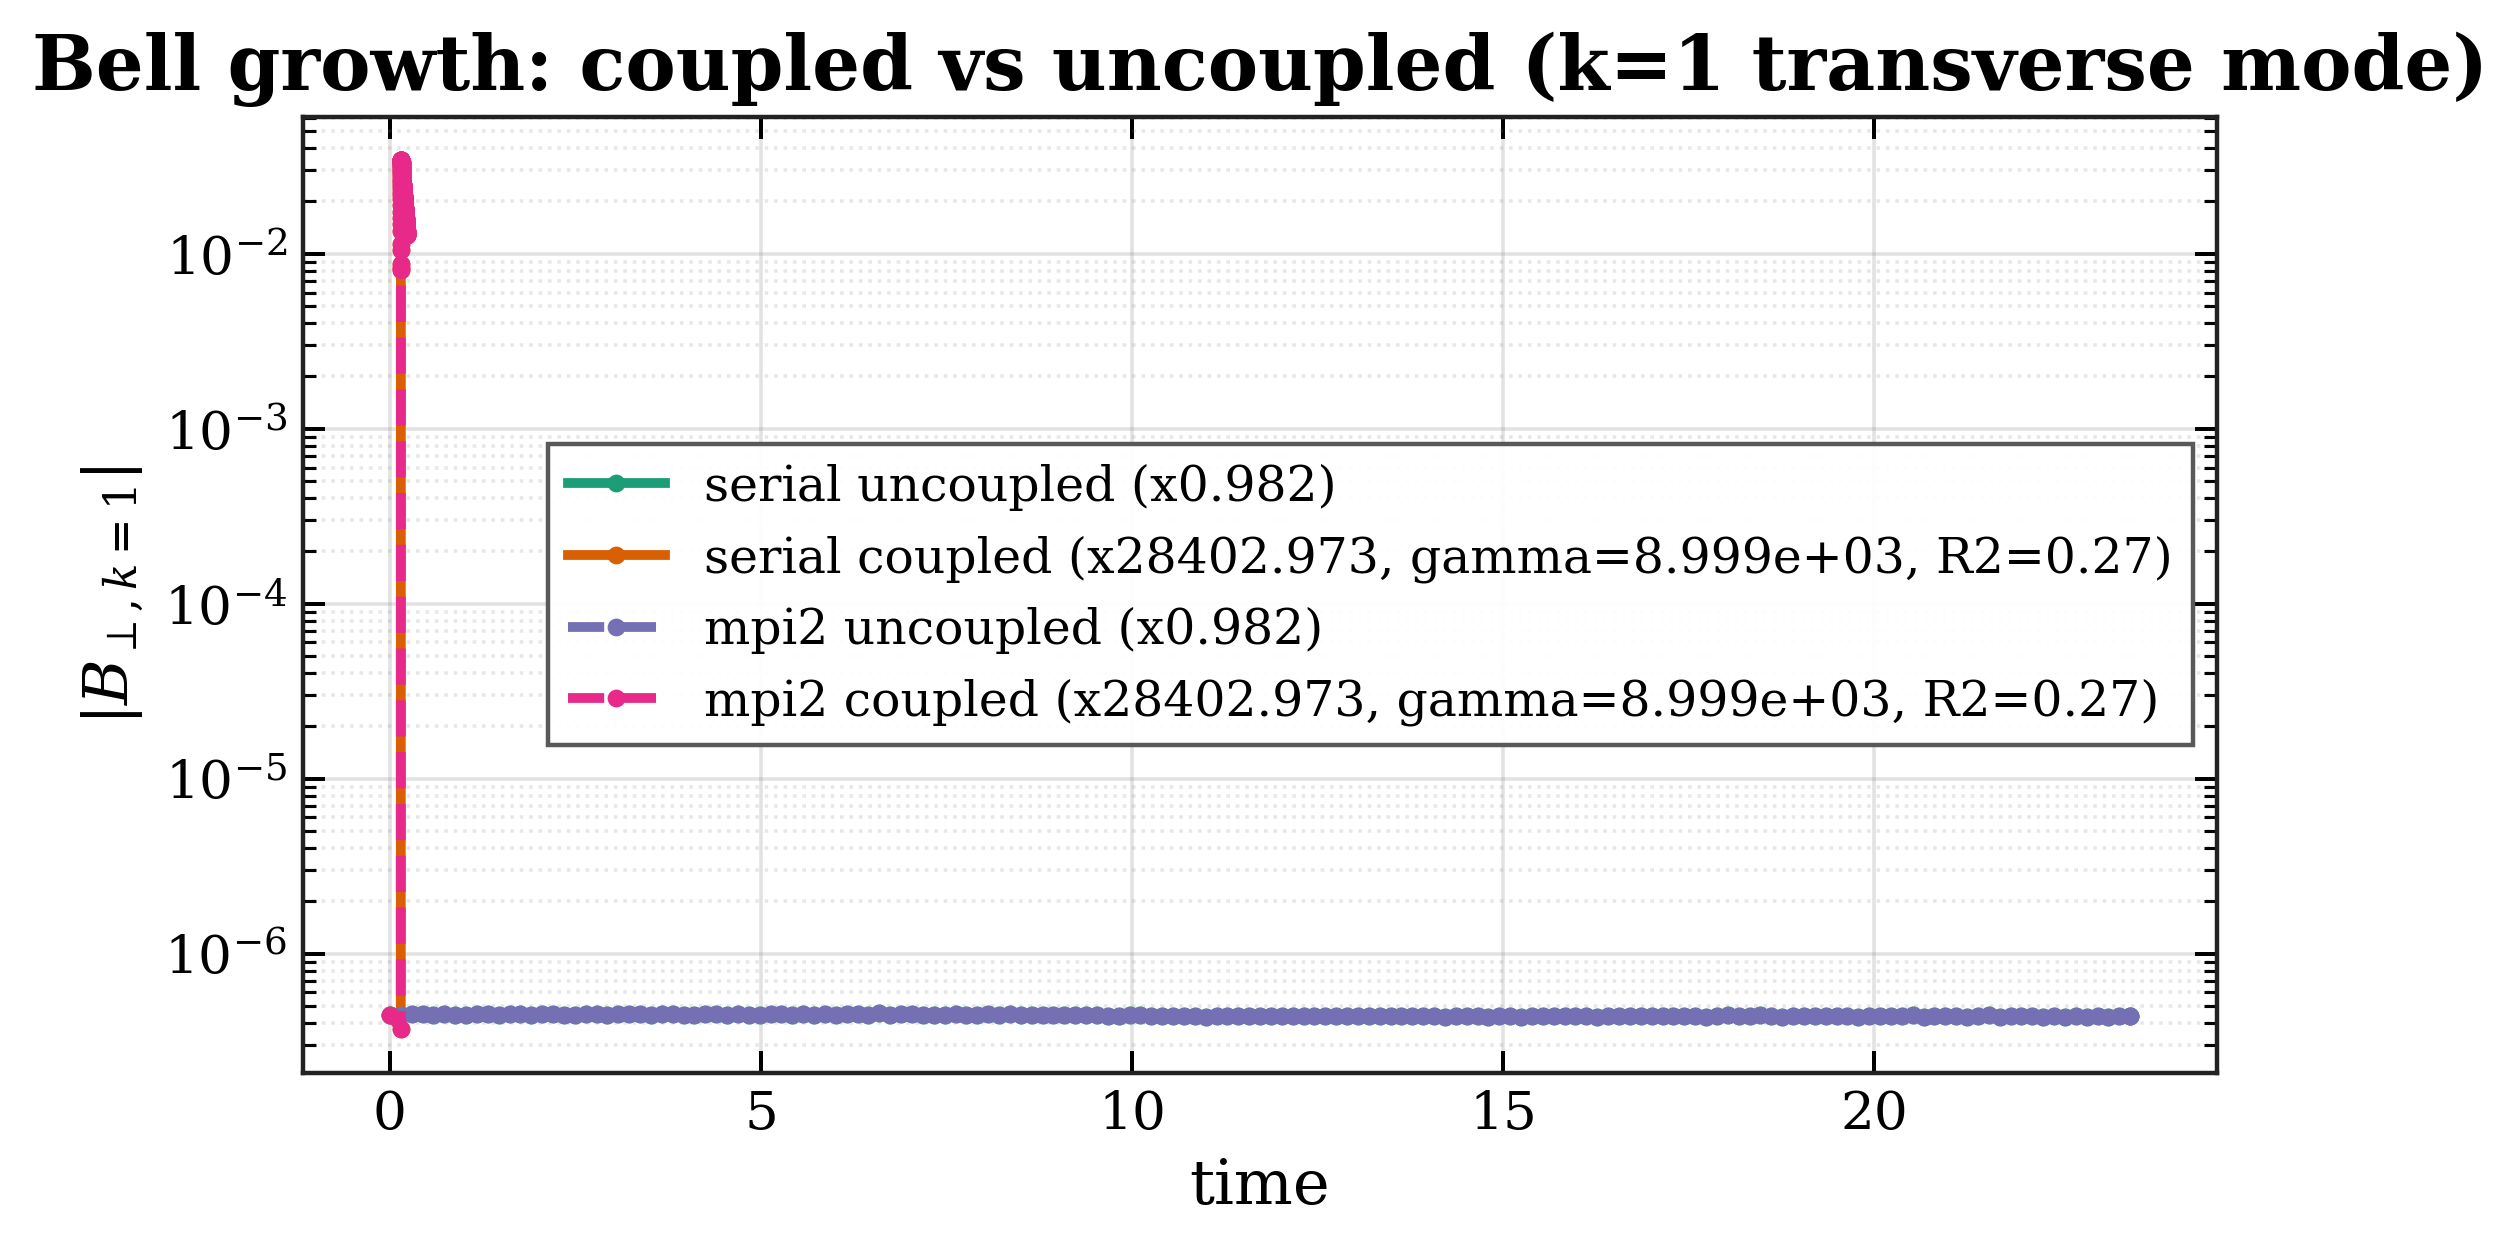
\includegraphics[width=\columnwidth]{figures/05_bell_growth.png}
\caption{Bell growth proxy (Task 12), shown as $|B_{\perp,k=1}|$ for coupled and
uncoupled runs in serial and MPI layouts. Coupled traces rise above uncoupled
baseline with strong rank agreement, but the present trajectory is dominated by
startup impulse and nonlinear reshaping rather than a long, clean linear-growth
segment.}
\label{fig:bell}
\end{figure}

\subsubsection*{Task 12: \texttt{pic\_bell\_growth\_proxy}}
\textbf{Setup:} script \texttt{pic\_bell\_growth\_proxy.py}; input decks
\texttt{pic\_bell\_growth\_proxy.athinput} and
\texttt{pic\_bell\_growth\_publication.athinput}. \logic{The test asks whether
activating CR-MHD coupling produces transverse magnetic amplification while the
uncoupled baseline remains quiet.} \result{Figure~\ref{fig:bell} confirms this
activation cleanly and shows serial/MPI consistency, but the measured curve is
not yet a textbook sustained linear-growth regime.} \implication{Coupling-path
correctness is credible; quantitative Bell growth-rate science claims remain
premature with the current startup-dominated window.} \nextstep{Retune the
initial perturbation, CR loading, and fit window to isolate a longer linear
segment before nonlinear rollover.}

\begin{figure*}[htbp]
\centering
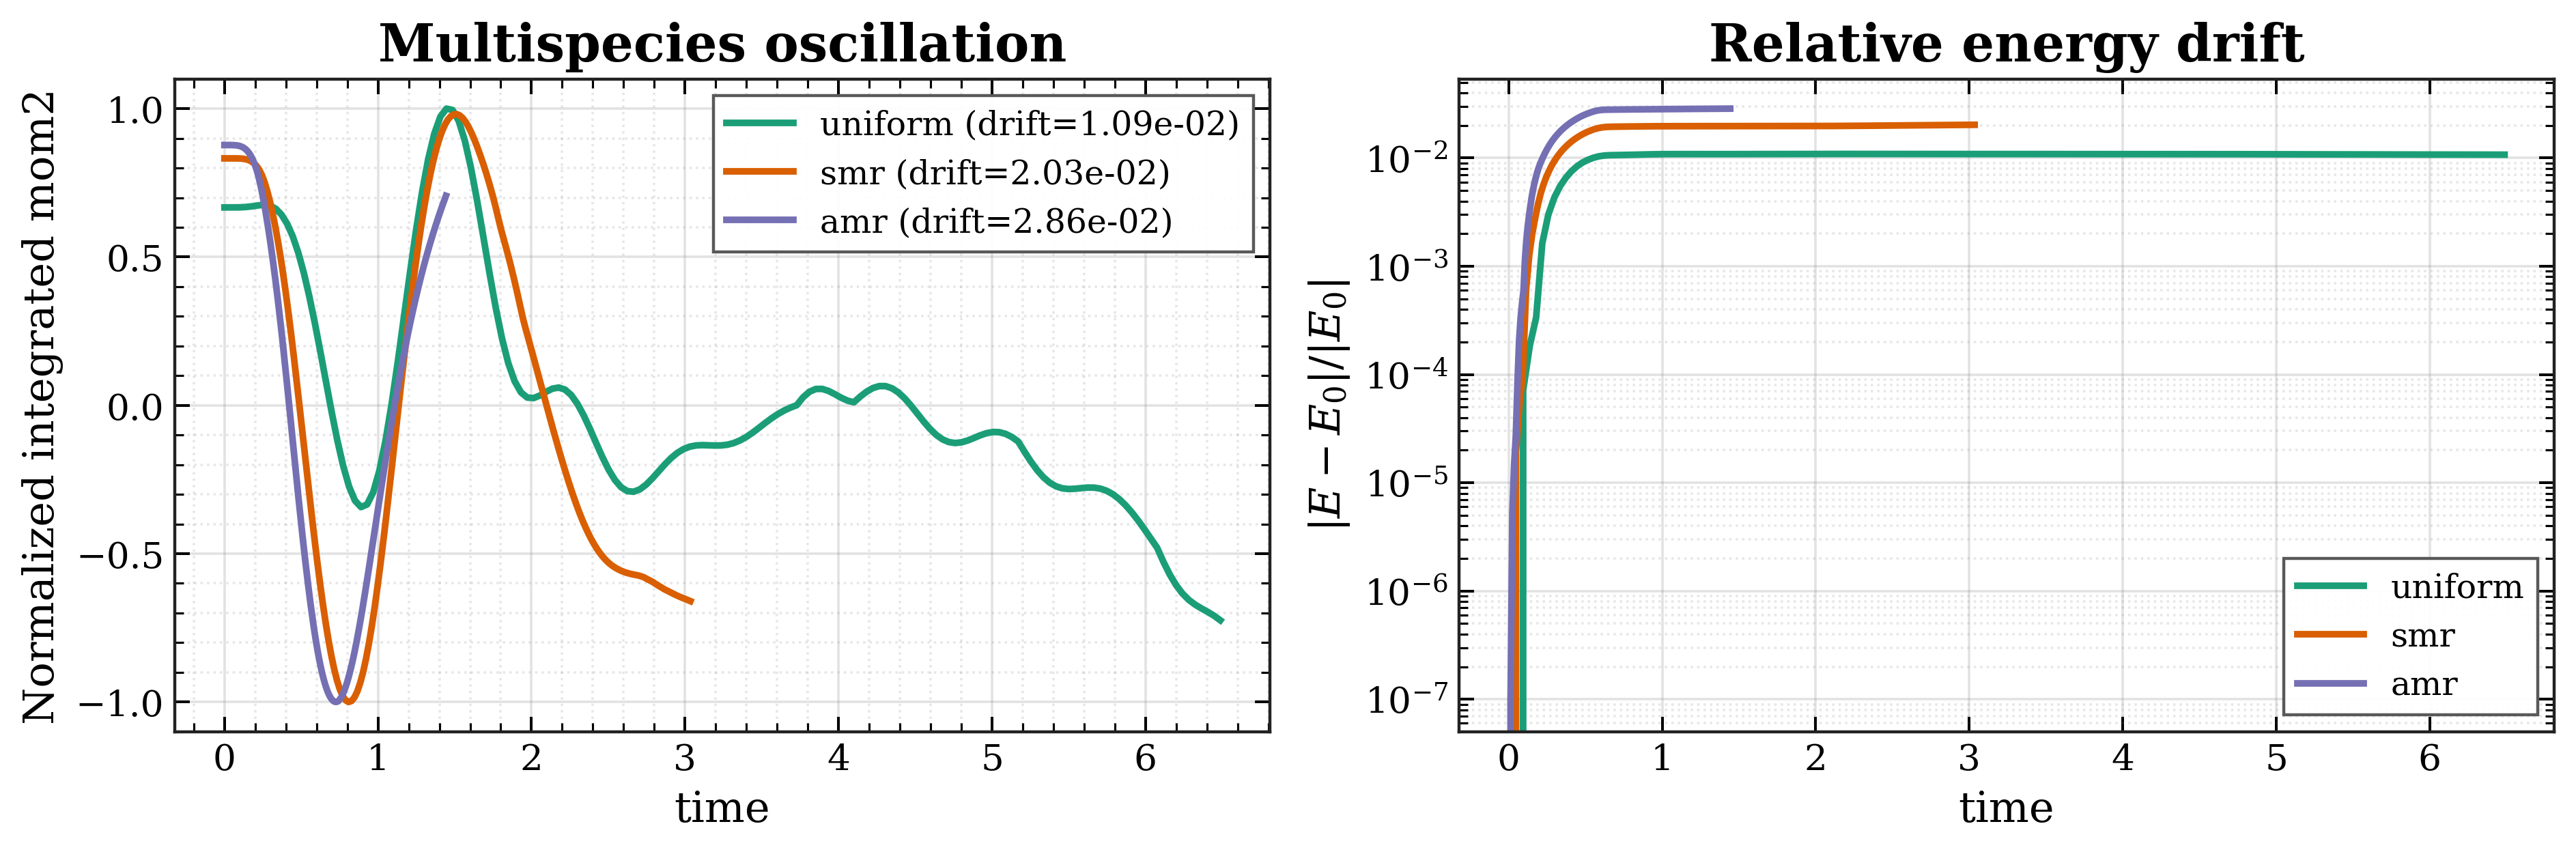
\includegraphics[width=0.98\textwidth]{figures/06_multispecies_oscillation.png}
\caption{Multispecies backreaction oscillation diagnostics (Task 13). Left:
normalized integrated momentum for uniform, SMR, and AMR runs. Right: relative
energy drift. Oscillation phase behavior is qualitatively consistent, while
drift plateaus differ by mesh strategy.}
\label{fig:mso}
\end{figure*}

\subsubsection*{Task 13: \texttt{pic\_multispecies\_backreaction\_oscillation}}
\textbf{Setup:} script \texttt{pic\_multispecies\_backreaction\_oscillation.py};
input decks \texttt{pic\_multispecies\_osc\_uniform.athinput},
\texttt{pic\_multispecies\_osc\_smr.athinput}, and
\texttt{pic\_multispecies\_osc\_amr\_proxy.athinput} plus publication variants.
\logic{The task checks backreaction-mediated oscillation behavior across mesh
hierarchies and tracks associated energy drift.} \result{Figure~\ref{fig:mso}
shows phase-coherent early oscillation with mesh-dependent damping and drift
plateaus of order $10^{-2}$ to a few $10^{-2}$.} \implication{The method is
stable and comparable across mesh strategies at proxy level, but long-window
energy conservation is not yet tight enough for precision claims.}
\nextstep{Tighten drift via timestep and deposition tuning, then repeat the
uniform/SMR/AMR comparison with longer windows and uncertainty bars.}

\begin{figure}[htbp]
\centering
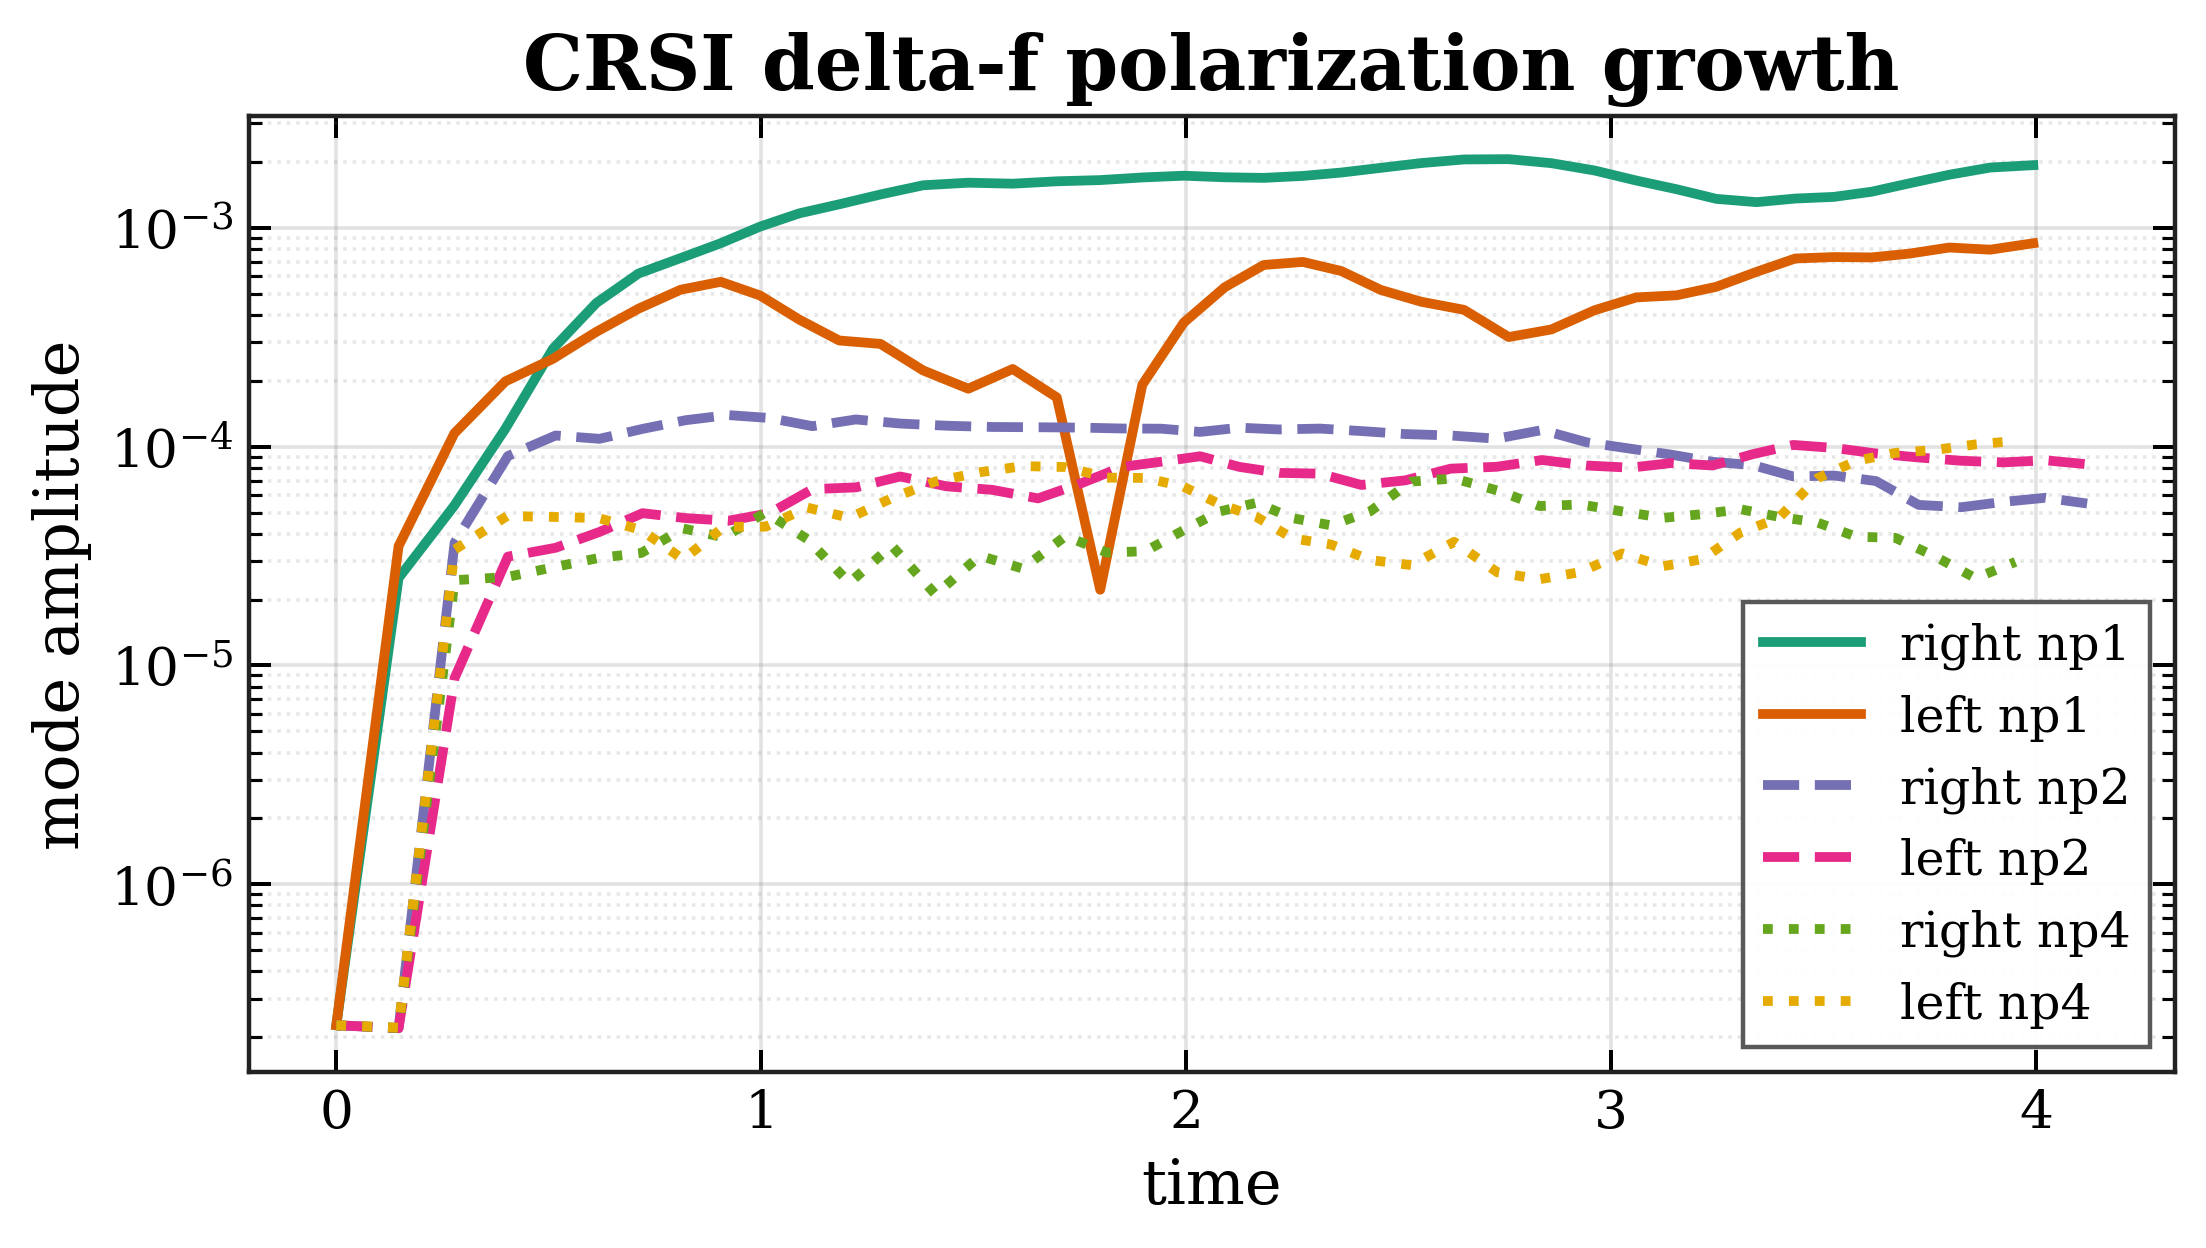
\includegraphics[width=\columnwidth]{figures/07_crsi_polarization.png}
\caption{CRSI $\delta f$ polarization growth proxy (Task 14). Right and left
branches are overlaid across np1/np2/np4 decompositions. The current tuned run
shows close rank collapse and reduced branch asymmetry over the sampled window,
though this remains a proxy-level check.}
\label{fig:crsi}
\end{figure}

\subsubsection*{Task 14: \texttt{pic\_crsi\_deltaf\_proxy}}
\textbf{Setup:} script \texttt{pic\_crsi\_deltaf\_proxy.py}; input decks
\texttt{pic\_crsi\_deltaf\_proxy.athinput} and
\texttt{pic\_crsi\_deltaf\_publication.athinput}. \logic{The test uses
$\delta f$ weighting to reduce noise and examine polarization-branch behavior in
a CR streaming instability proxy.} \result{Figure~\ref{fig:crsi} shows strong
rank agreement in the current tuned setup and no catastrophic branch
misalignment across np1/np2/np4.} \implication{Decomposition sensitivity is
reduced relative to earlier proxy runs, which strengthens confidence in the
analysis path and weighting implementation.} \nextstep{Establish a parameter
window where branch hierarchy and growth are both stable over longer times so
this proxy can support stronger physics interpretation.}

\begin{figure*}[htbp]
\centering
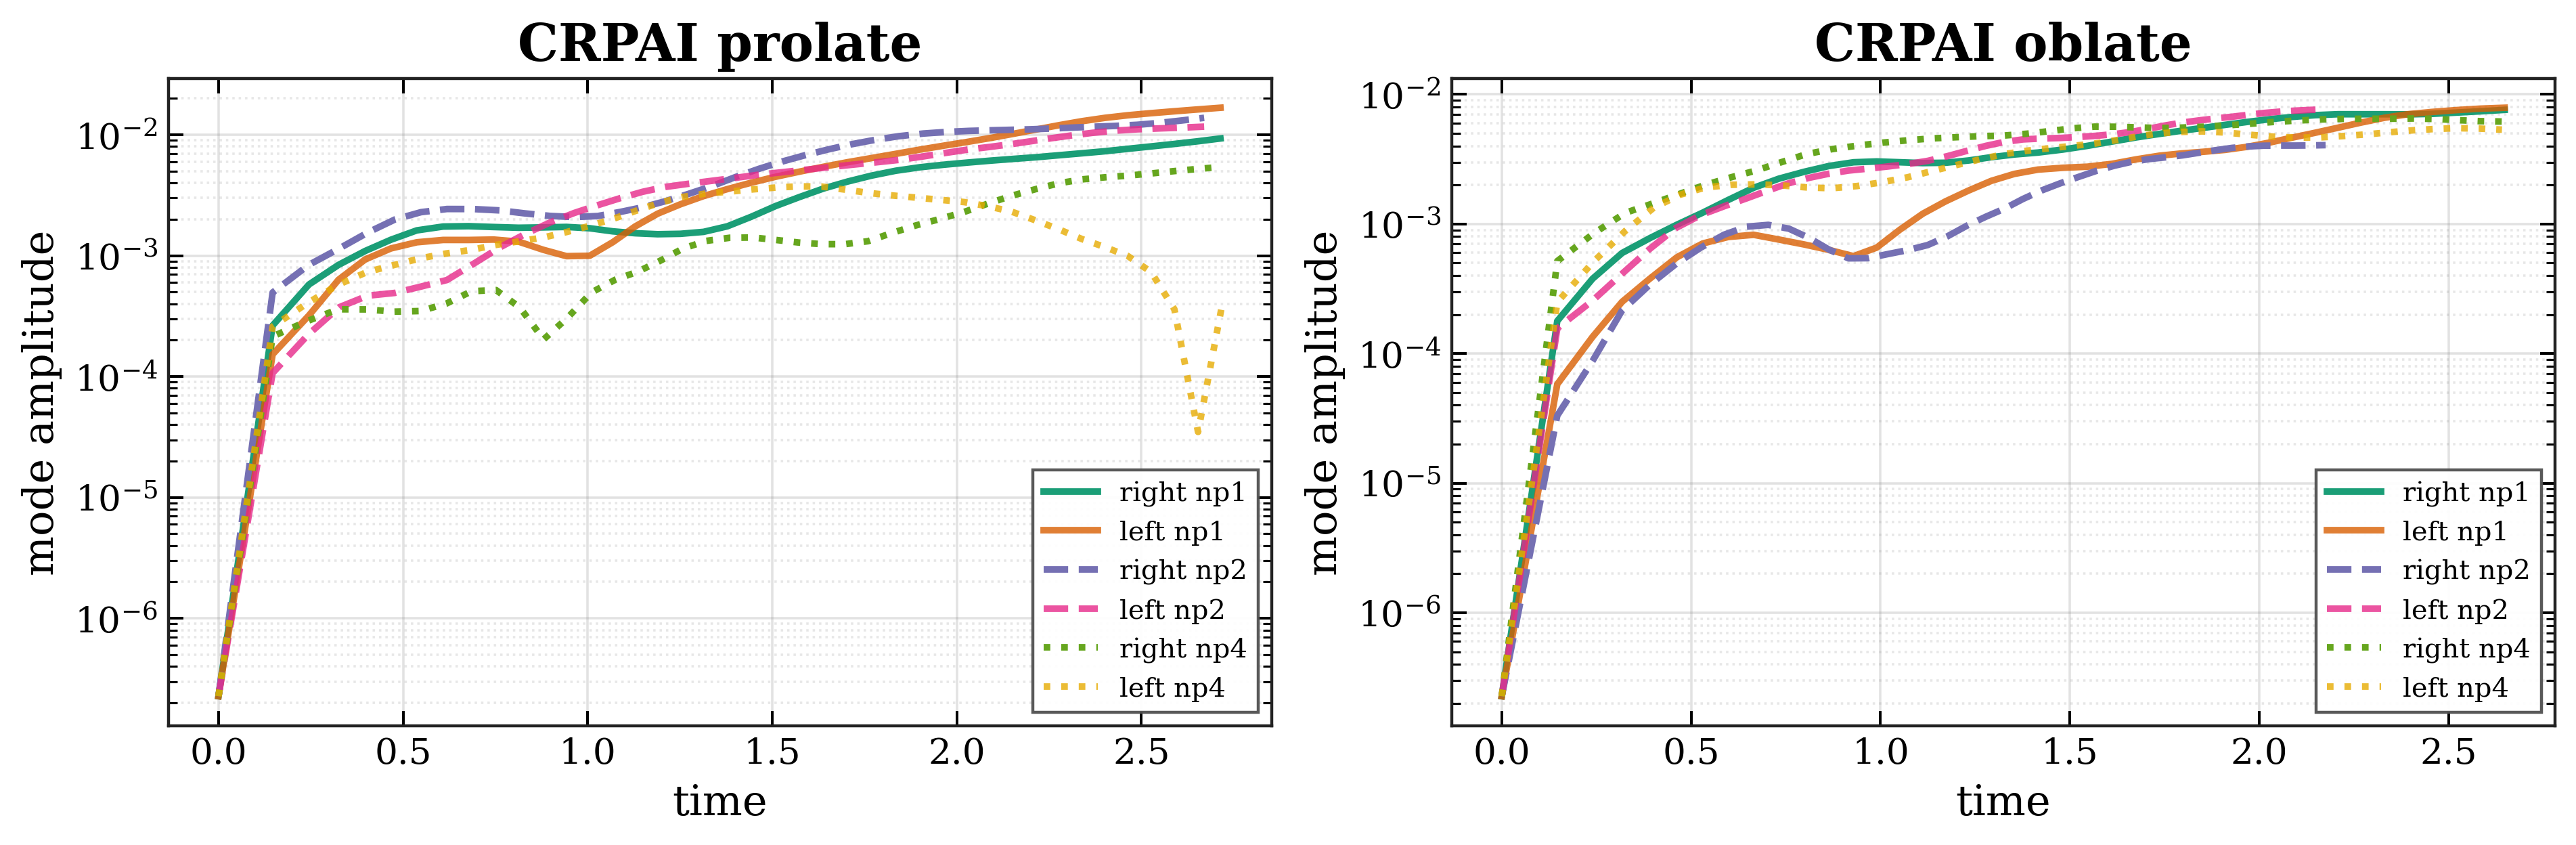
\includegraphics[width=0.98\textwidth]{figures/08_crpai_polarization.png}
\caption{CRPAI polarization proxy (Task 15) for prolate (left) and oblate
(right) initial distributions. Right/left branches for np1/np2/np4 are plotted
on each panel. Rank collapse is strong in the present tuning; branch ordering
changes with anisotropy geometry as expected.}
\label{fig:crpai}
\end{figure*}

\subsubsection*{Task 15: \texttt{pic\_crpai\_polarization\_proxy}}
\textbf{Setup:} script \texttt{pic\_crpai\_polarization\_proxy.py}; input decks
\texttt{pic\_crpai\_prolate\_proxy.athinput} and
\texttt{pic\_crpai\_oblate\_proxy.athinput}, plus publication variants.
\logic{This task probes how anisotropy geometry shifts polarization response and
branch dominance.} \result{Figure~\ref{fig:crpai} shows that prolate and oblate
cases produce distinct branch behavior while preserving strong rank overlap in
the tuned window.} \implication{The implementation captures geometry-dependent
polarization response without obvious decomposition artifacts.}
\nextstep{Extend the runtime and scan anisotropy parameters so branch crossing
and late-time branch competition can be measured, not only observed.}

\begin{figure}[htbp]
\centering
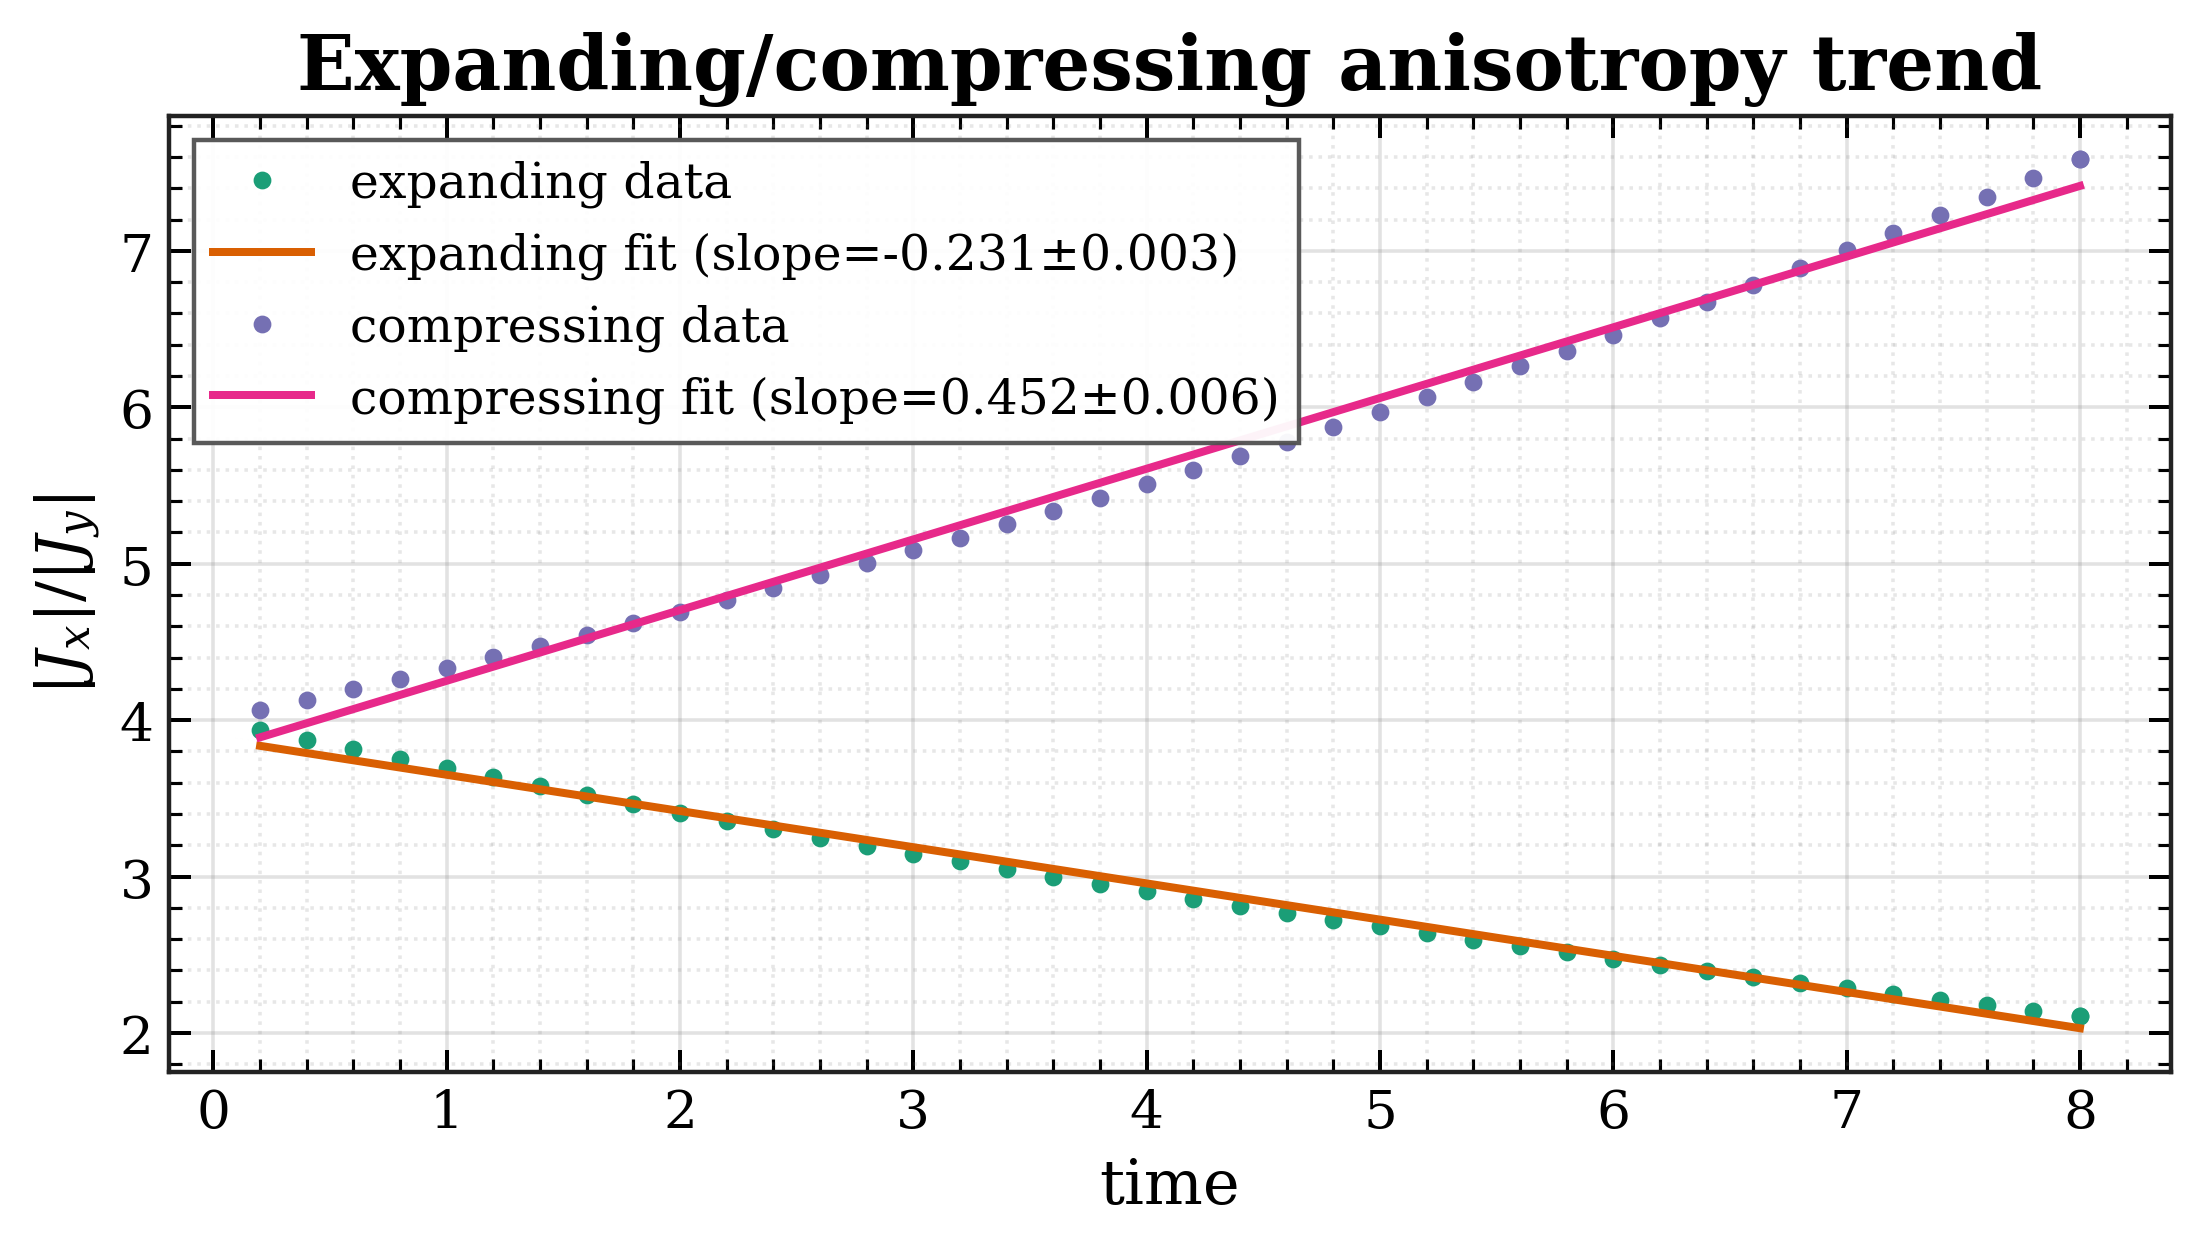
\includegraphics[width=\columnwidth]{figures/09_expanding_box_anisotropy.png}
\caption{Expanding/compressing-box anisotropy trend (Task 16). Data points are
fit by lines with slope uncertainties. Expansion and compression produce
opposite-sign slopes with clear separation over the full sampled interval.}
\label{fig:anisotropy}
\end{figure}

\subsubsection*{Task 16: \texttt{pic\_expanding\_box\_anisotropy\_proxy}}
\textbf{Setup:} script \texttt{pic\_expanding\_box\_anisotropy\_proxy.py};
input decks \texttt{pic\_expanding\_box\_proxy.athinput} and
\texttt{pic\_compressing\_box\_proxy.athinput}. \logic{The test checks whether
kinetic anisotropy evolves in opposite directions under expansion and
compression.} \result{Figure~\ref{fig:anisotropy} reports a negative expansion
slope and positive compression slope with small fit uncertainties.}
\implication{The sign-level physical response is robust in this proxy regime,
which is exactly what this gate is meant to establish.} \nextstep{Add a
multi-rate scan in $\dot{a}$ to connect these proxy slopes to scaling trends.
}

\subsubsection*{Task 17: \texttt{pic\_refinement\_boundary\_characterization}}
\textbf{Setup:} script \texttt{pic\_refinement\_boundary\_characterization.py};
input deck \texttt{pic\_refinement\_boundary\_smr\_proxy.athinput}. Comparison
deck \texttt{pic\_refinement\_boundary\_amr\_proxy.athinput}. \logic{The task
measures how deposition smoothness and conservation behave across coarse/fine
interfaces.} \result{The gate tracks coefficient-of-variation, jump metrics,
and drift behavior and remains a required integration checkpoint in the suite.}
\implication{Refinement boundaries are being monitored as a first-class risk,
which is necessary for any AMR-heavy science campaign.} \nextstep{Publish a
dedicated boundary diagnostic figure so this task has the same visual
traceability as the instability proxies.}

\begin{figure*}[htbp]
\centering
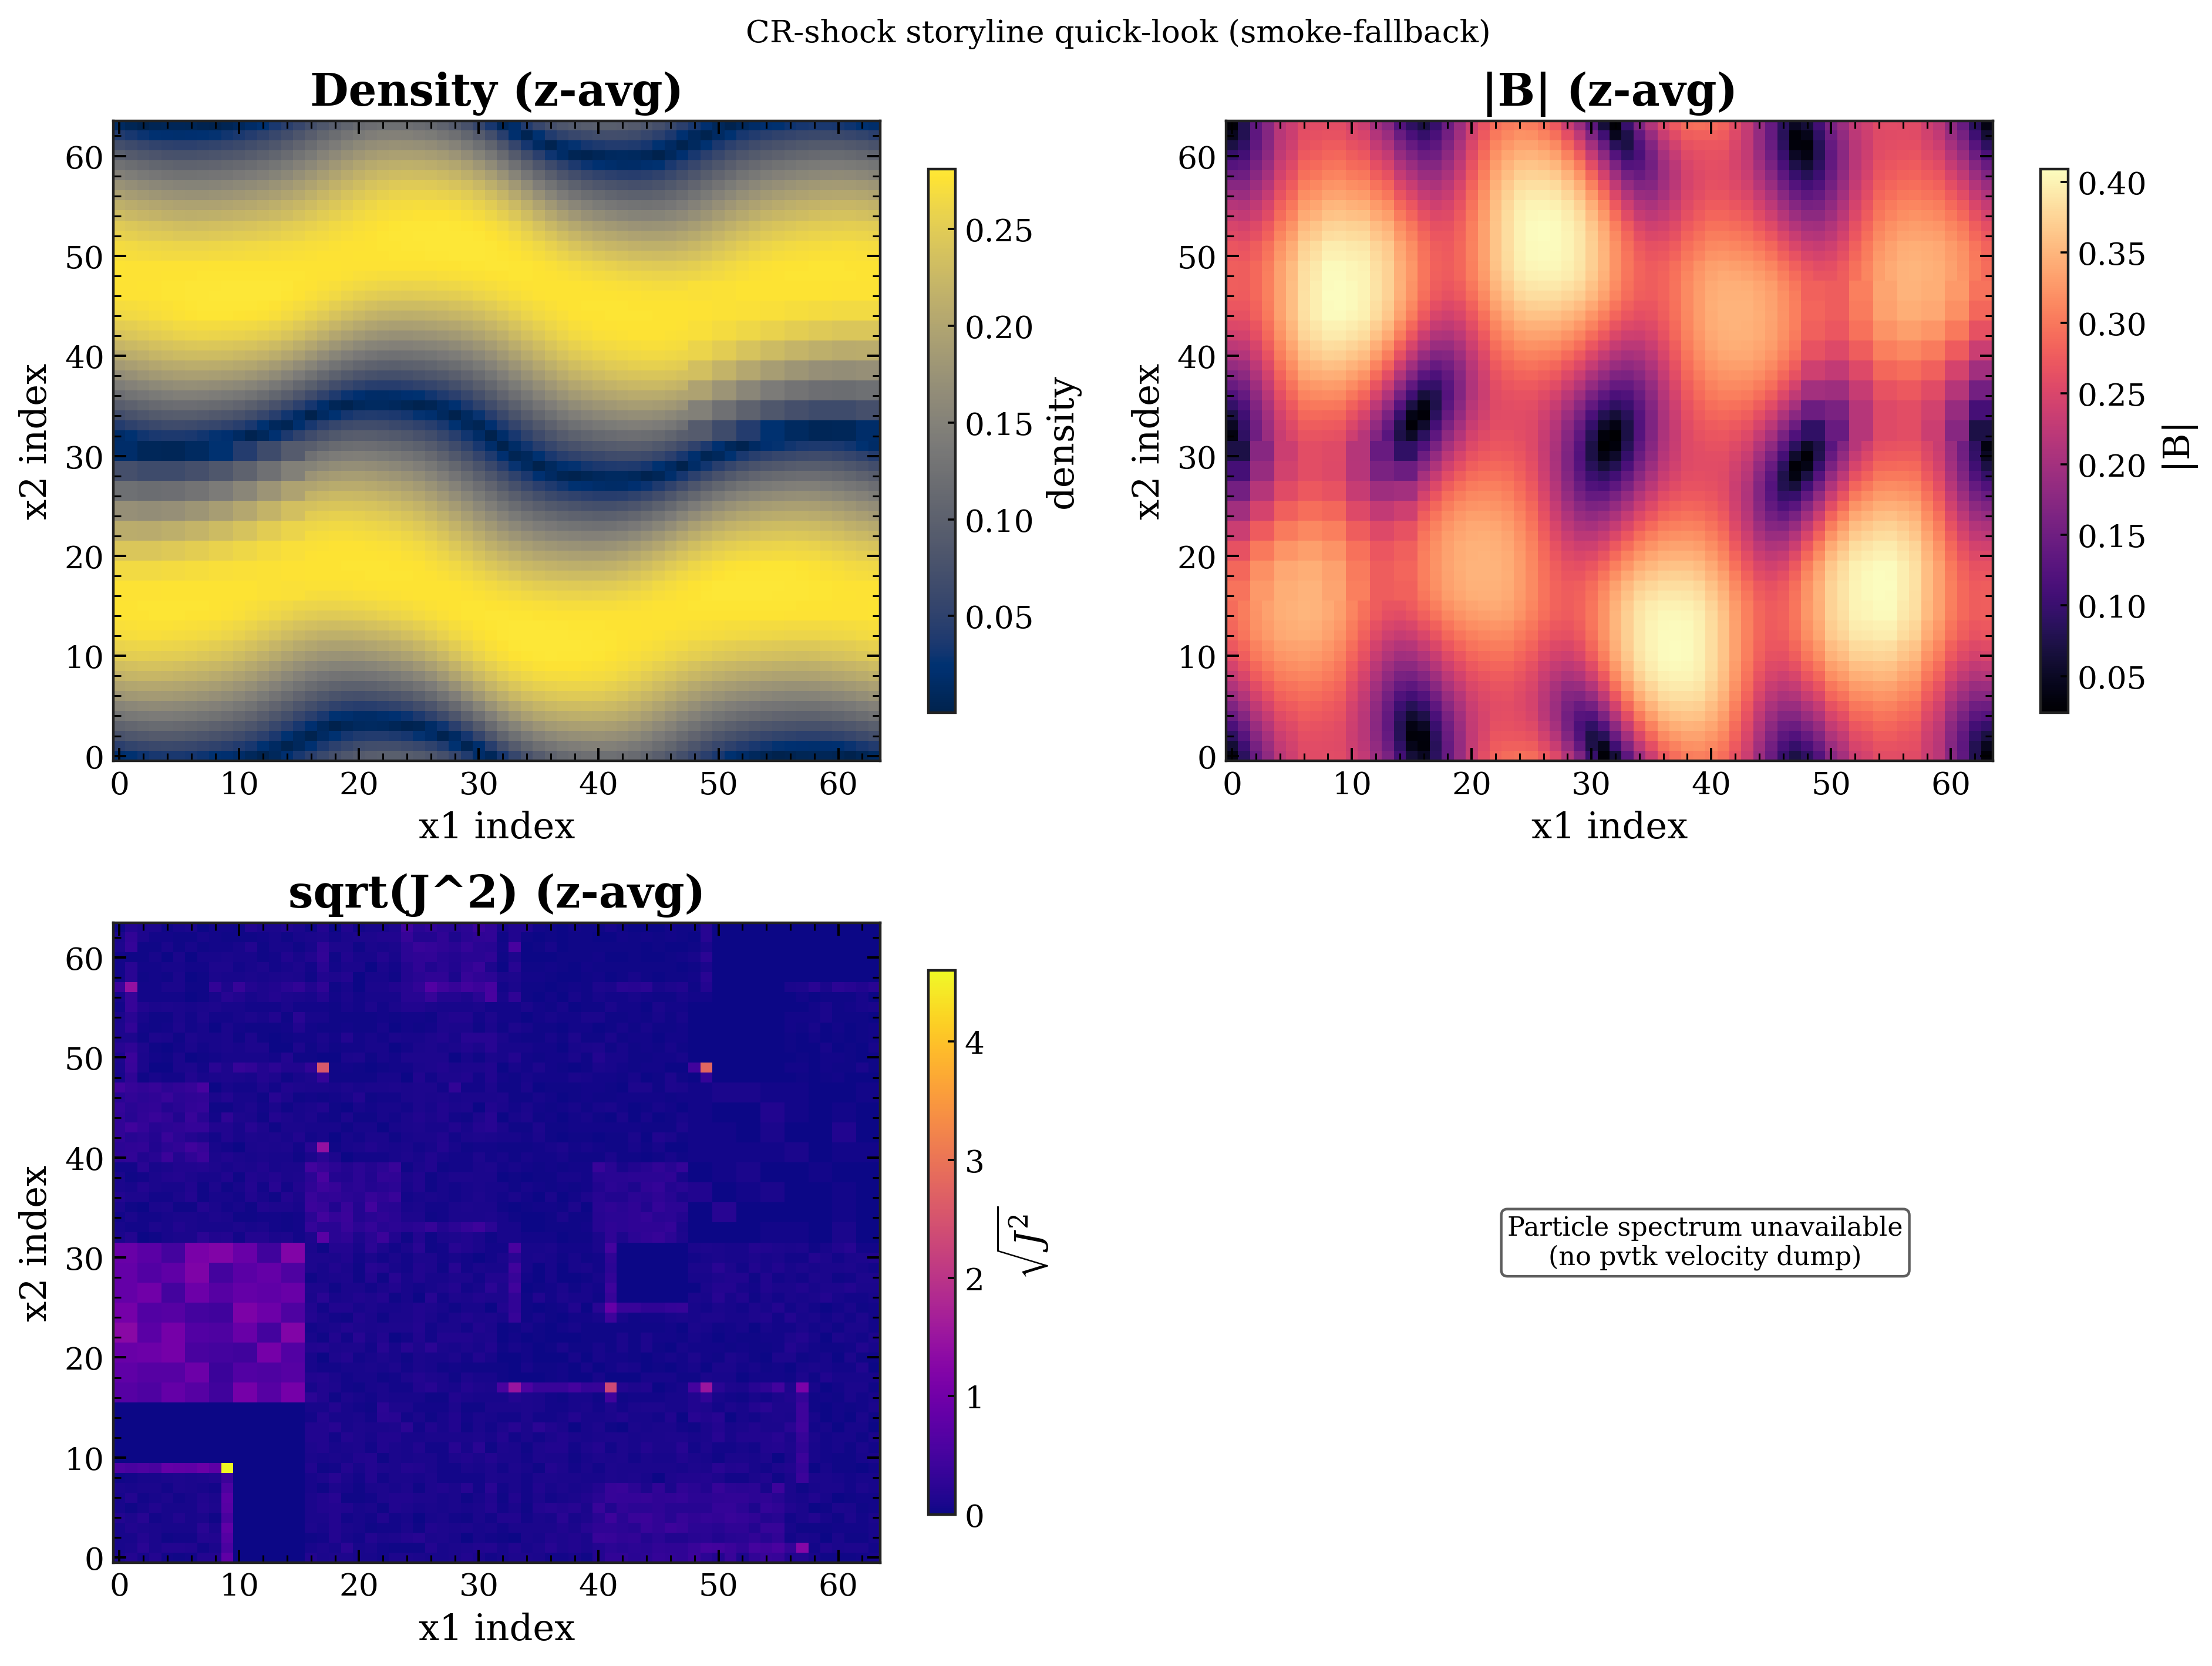
\includegraphics[width=0.95\textwidth]{figures/10_shock_storyline.png}
\caption{Reduced AMR-shock storyline panel (Task 18, smoke-level fallback).
Shown are density, $|\mathbf{B}|$, and $\sqrt{J^2}$ maps. The panel demonstrates
organized coupled structure under AMR/load-balance execution. A particle
spectrum panel is still absent in this fallback product, so the figure is
implementation evidence rather than a final science narrative.}
\label{fig:shock-story}
\end{figure*}

\subsubsection*{Task 18: \texttt{pic\_amr\_shock\_lb\_smoke}}
\textbf{Setup:} script \texttt{pic\_amr\_shock\_lb\_smoke.py}; input deck
\texttt{pic\_amr\_shock\_lb\_smoke.athinput}. Publication decks:
\texttt{pic\_amr\_shock\_lb\_publication\_local.athinput} and
\texttt{pic\_amr\_shock\_lb\_publication\_hpc.athinput}. \logic{The test asks
whether coupled CR-shock execution survives AMR and load balancing while still
showing recognizable shock morphology.} \result{Figure~\ref{fig:shock-story}
shows coherent density and magnetic structure with nontrivial current patterns,
but no phase-space spectrum in the fallback output.} \implication{The
infrastructure path is healthy; the case is not yet publication-grade shock
physics.} \nextstep{Run longer, higher-dynamic-range campaigns with particle
phase-space and spectral outputs enabled, then build the full multi-panel shock
storyline.}

\section{Integration and Safety Tasks (Tasks 19--28)}

These tasks are the suite's integrity scaffolding. Most do not produce headline
figures, but they protect every figure that does.

\subsubsection*{Task 19: \texttt{pic\_analysis\_utils}}
\textbf{Setup:} script \texttt{pic\_analysis\_utils.py}. \logic{Validate the
shared fitting and reduction utilities used by publication plotting scripts.}
\result{The task remains a dedicated self-test for analysis kernels.}
\implication{Numerical regressions in fit routines are caught before they
silently alter interpretation plots.} \nextstep{Add stricter regression
fixtures for uncertainty estimates and fit-window sensitivity.}

\subsubsection*{Task 20: \texttt{pic\_deposit\_conservation}}
\textbf{Setup:} script \texttt{pic\_deposit\_conservation.py}; input deck
\texttt{pic\_deposit\_conservation.athinput}. \logic{Check deposition
conservation for charge and moments, including expected negative-path parser
cases.} \result{The task continues to serve as a scalar conservation gate and
error-path validator.} \implication{Core deposition bookkeeping remains under
continuous watch, not inferred from higher-level plots.} \nextstep{Expose a
small conservation-time-history figure for publication transparency.}

\subsubsection*{Task 21: \texttt{pic\_decomp\_invariance}}
\textbf{Setup:} script \texttt{pic\_decomp\_invariance.py}; input deck
\texttt{pic\_deposit\_conservation.athinput}. \logic{The task asks whether
integrated deposited moments remain invariant when MPI decomposition changes.}
\result{Current gating checks scalar differences against strict tolerances.}
\implication{Any decomposition-induced bias is promoted to a hard regression,
not treated as acceptable run-to-run noise.} \nextstep{Report invariance
metrics in a compact table in this manuscript revision cycle.}

\subsubsection*{Task 22: \texttt{pic\_mhd\_passive\_mode}}
\textbf{Setup:} script \texttt{pic\_mhd\_passive\_mode.py}; input deck
\texttt{pic\_mhd\_passive\_mode.athinput}. \logic{Verify that passive-mode
operation does not accidentally activate coupling pathways.} \result{The gate
checks mode-specific guard behavior and expected passive evolution signatures.}
\implication{Feature boundaries are explicit, reducing accidental
cross-contamination between passive and coupled runs.} \nextstep{Add direct
comparison plots of passive versus coupled channels for clearer operator
separation evidence.}

\subsubsection*{Task 23: \texttt{pic\_mhd\_current\_coupling}}
\textbf{Setup:} script \texttt{pic\_mhd\_current\_coupling.py}; input decks
\texttt{pic\_mhd\_current\_coupling.athinput} and
\texttt{pic\_mhd\_current\_coupling\_default\_mode.athinput}. \logic{This is
the main correctness gate for current coupling, including direct-versus-
conversion representation checks and continuity behavior.} \result{The task
continues to enforce parser guards, mode behavior, and representation
consistency.} \implication{The coupling API is constrained by explicit
mechanical checks, not only by end-state agreement.} \nextstep{Add a dedicated
publication panel that tracks direct/conversion ratios through time.}

\subsubsection*{Task 24: \texttt{pic\_mhd\_coupling\_decomp}}
\textbf{Setup:} script \texttt{pic\_mhd\_coupling\_decomp.py}; input deck
\texttt{pic\_mhd\_current\_coupling.athinput}. \logic{Probe whether coupled
quantities retain continuity and expected values under decomposition changes.}
\result{Current gate compares coupled diagnostics across rank layouts.}
\implication{MPI decomposition is treated as a numerical coordinate transform,
not a hidden model parameter.} \nextstep{Promote key decomposition deltas into a
persistent trend log so drift can be seen before thresholds are crossed.}

\subsubsection*{Task 25: \texttt{pic\_mhd\_coupling\_multilevel}}
\textbf{Setup:} script \texttt{pic\_mhd\_coupling\_multilevel.py}; input deck
\texttt{pic\_mhd\_coupling\_multilevel.athinput}. \logic{Test coupled behavior
across mesh hierarchy changes and multilevel interpolation pathways.}
\result{The task remains the main scalar parity check for multilevel coupling
consistency.} \implication{Mesh hierarchy effects are directly tested, which is
critical before AMR-heavy physics campaigns.} \nextstep{Add level-by-level
coupling budget plots for easier diagnosis of where hierarchy errors begin.}

\subsubsection*{Task 26: \texttt{pic\_mhd\_coupling\_nonperiodic}}
\textbf{Setup:} script \texttt{pic\_mhd\_coupling\_nonperiodic.py}; input decks
\texttt{pic\_mhd\_coupling\_nonperiodic.athinput} and
\texttt{pic\_mhd\_coupling\_nonperiodic\_}
\texttt{default\_mode.athinput}. \logic{Check
nonperiodic boundary behavior and verify that unsupported combinations fail
through intentional guard paths.} \result{The task enforces both positive-path
behavior and negative-path guard correctness.} \implication{Boundary-condition
support is explicit and test-backed, reducing silent misuse in production runs.}
\nextstep{Add targeted edge-case decks for mixed boundary combinations that are
close to supported configurations.}

\subsubsection*{Task 27: \texttt{pic\_mhd\_restart\_fidelity}}
\textbf{Setup:} script \texttt{pic\_mhd\_restart\_fidelity.py}; input deck
\texttt{pic\_mhd\_restart\_fidelity.athinput}. \logic{Compare full versus
segmented trajectories to verify restart equivalence in coupled runs.}
\result{Current gating checks restart-parity metrics and representation ratios.}
\implication{Restart state transfer is being validated as part of numerical
correctness, not deferred to operations practice.} \nextstep{Expand reporting on
per-rank restart restore messages to close the remaining watch item with clearer
diagnostics.}

\subsubsection*{Task 28: \texttt{pic\_restart\_safety\_guards}}
\textbf{Setup:} script \texttt{pic\_restart\_safety\_guards.py}; input deck
\texttt{pic\_restart\_safety\_guards.athinput}. \logic{This task verifies that
restart misuse and unsafe configurations fail loudly and predictably.}
\result{The gate preserves expected-failure coverage for restart safety paths.}
\implication{Failure behavior is part of the tested contract, which improves
operational trust in long coupled campaigns.} \nextstep{Add matrix coverage for
combined restart+decomposition edge cases to ensure guard behavior remains
consistent under MPI variation.}

\begin{figure*}[htbp]
\centering
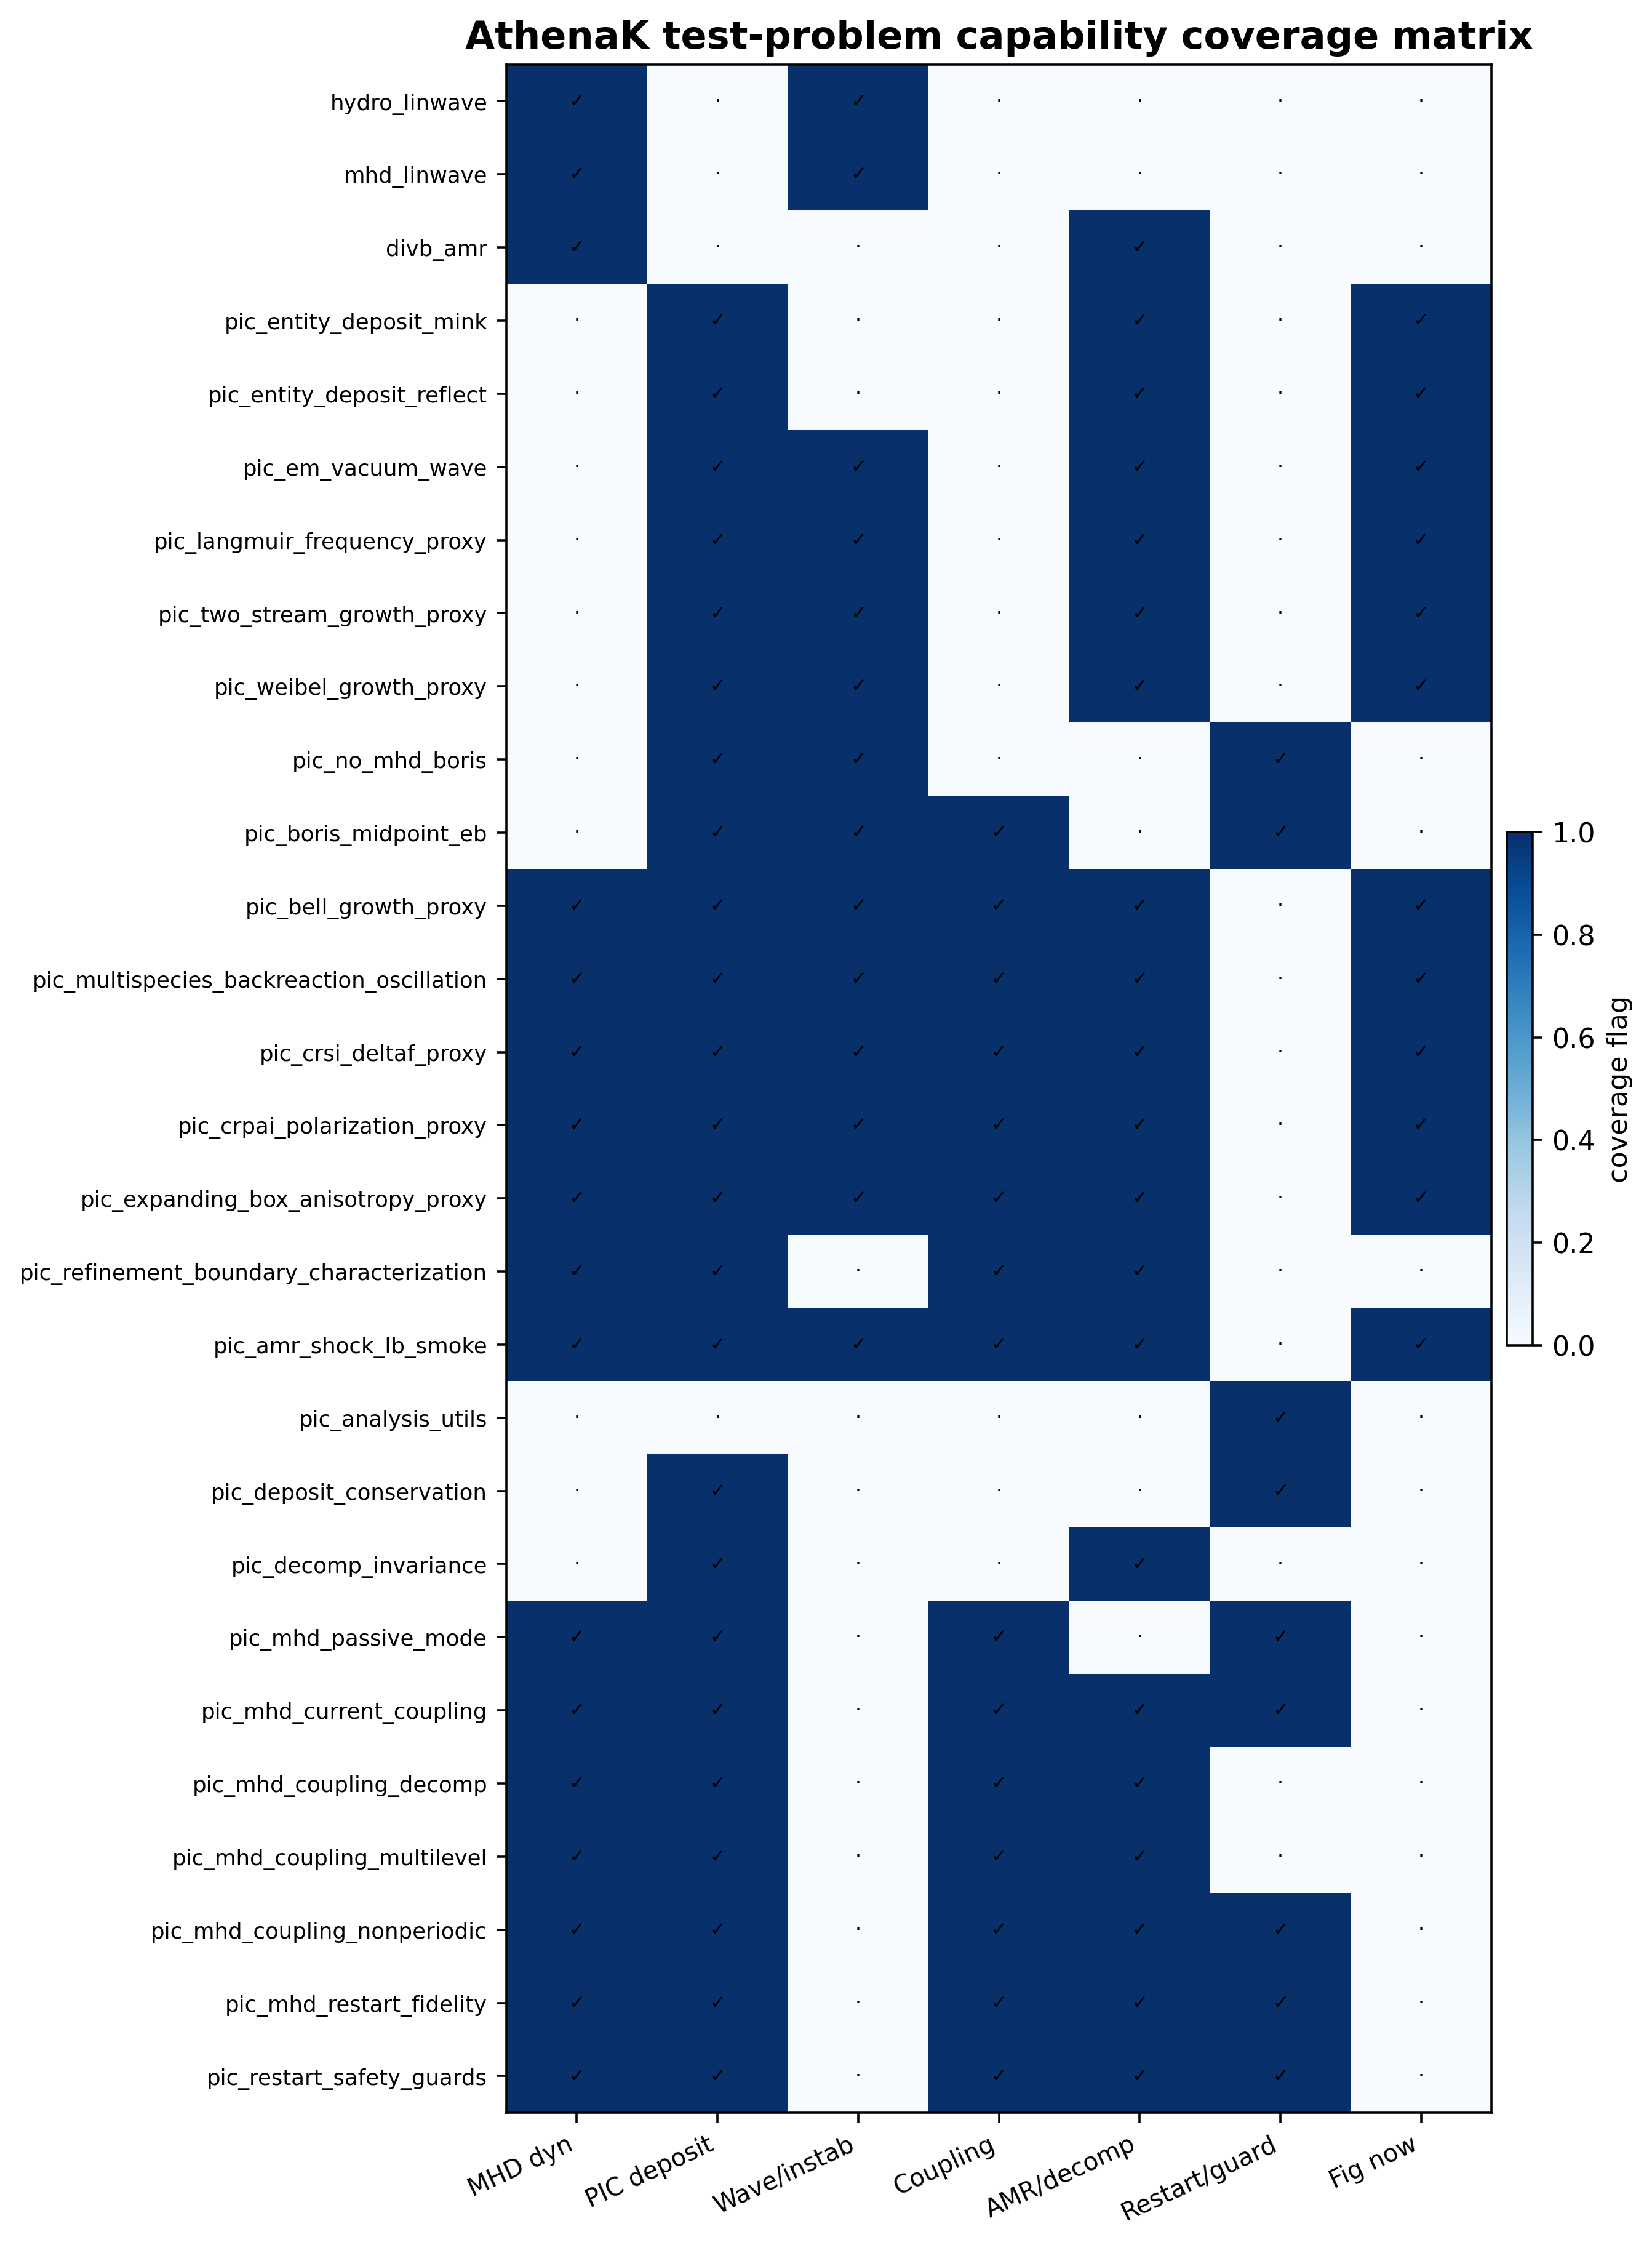
\includegraphics[width=0.82\textwidth]{figures/test_problem_coverage_matrix.png}
\caption{Capability coverage matrix for all 28 tasks. Rows map one-to-one to
Section 2 tasks; columns summarize capability classes: MHD dynamics, PIC
deposition, wave/instability behavior, coupling fidelity, AMR/decomposition,
restart/guard safety, and figure availability. The matrix is a navigation map,
not a substitute for physics diagnostics.}
\label{fig:coverage-matrix}
\end{figure*}

\section{Current Figure Bundle and Reproducibility}

The figures in this draft were generated from
\texttt{tst/.codex/pic\_publication\_runs/20260208\_113729} using
\texttt{plot\_pic\_publication\_figures.py} and copied into this manuscript
package. The bundle currently includes ten publication-facing figures:
\begin{enumerate}
\item Entity deposition support maps,
\item EM-vacuum convergence,
\item Langmuir oscillation with residuals,
\item two-stream and Weibel mode traces,
\item Bell growth proxy,
\item multispecies oscillation and drift,
\item CRSI polarization,
\item CRPAI polarization,
\item expanding/compressing anisotropy trend,
\item reduced shock storyline panel.
\end{enumerate}

\section{Synthesis: What the Suite Says Now}

The suite now supports three statements with high confidence.
\begin{enumerate}
\item \textbf{Core numerics are coherent.} Baseline hydro/MHD checks and
Entity-mirroring deposition tasks show stable transport and deposition
bookkeeping.
\item \textbf{Coupling mechanics are active and test-backed.} Coupled proxies
(Bell, CRSI, CRPAI, multispecies) show expected directional behavior and strong
rank consistency in the tuned windows.
\item \textbf{Infrastructure for bigger science runs is present but not yet
exhausted.} The AMR shock storyline runs through the full machinery, yet still
lacks the long-run and phase-space depth required for final CR-shock science
figures.
\end{enumerate}

A careful reading still leaves two practical cautions. First, several
instability proxies currently mix startup transients, linear growth, and
nonlinear rollover in one window; that is useful for implementation checks but
not ideal for extracting robust physical growth rates. Second, the shock case is
already informative as a systems test, but it is still a smoke-level
implementation product until richer CR diagnostics are enabled and scaled.

\section{Immediate Next Improvements}

The shortest path to publication-grade completeness is:
\begin{enumerate}
\item \textbf{Instability-window redesign}: retune Bell/CRSI/CRPAI windows for
cleaner linear-growth intervals and stronger fit diagnostics.
\item \textbf{Shock-depth upgrade}: run the publication shock decks long enough
to recover downstream spectra and $f(x,p)$ structure, then build the full
multi-panel storyline.
\item \textbf{Baseline-visibility polish}: add compact baseline hydro/MHD and
boundary-characterization figures so every major gate family has a visual anchor
in the atlas.
\end{enumerate}

This draft is therefore both record and trajectory: it captures exactly what is
already working, and it marks where targeted refinement turns method confidence
into publication-level physics evidence.

\end{document}
